\documentclass[12pt, a4paper]{memoir} % for a short document
\usepackage[english]{babel}

\usepackage [vscale=0.76,includehead]{geometry}                % See geometry.pdf to learn the layout options. There are lots.
%\geometry{a4paper}                   % ... or a4paper or a5paper or ... 
%\geometry{landscape}                % Activate for for rotated page geometry
%\OnehalfSpacing
% \setSingleSpace{1.05}
%\usepackage[parfill]{parskip}
\usepackage{longtable}
\usepackage{algorithm}
\usepackage{subfig}
\usepackage[noend]{algpseudocode}    % Activate to begin paragraphs with an empty line rather than an indent
\usepackage{graphicx}
\usepackage{amsmath}
\usepackage{fullpage}
\usepackage{mathptmx} % font = times
\usepackage{helvet} % font sf = helvetica
\usepackage[utf8]{inputenc} % Required for inputting international characters
\usepackage[T1]{fontenc}
\usepackage{relsize}
\usepackage{hyperref}
%Style des t�tes de section, headings, chapitre
\headstyles{komalike}
\nouppercaseheads
\chapterstyle{dash}
\makeevenhead{headings}{\sffamily\thepage}{}{\sffamily\leftmark} 
\makeoddhead{headings}{\sffamily\rightmark}{}{\sffamily\thepage}
\makeoddfoot{plain}{}{}{} % Pages chapitre. 
\makeheadrule{headings}{\textwidth}{\normalrulethickness}
%\renewcommand{\leftmark}{\thechapter ---}
\renewcommand{\chaptername}{\relax}
\renewcommand{\chaptitlefont}{ \sffamily\bfseries \LARGE}
\renewcommand{\chapnumfont}{ \sffamily\bfseries \LARGE}
\setsecnumdepth{subsection}
\usepackage[backend=bibtex,
style=numeric,
bibencoding=ascii
%style=alphabetic
%style=reading
]{biblatex}
\addbibresource{example.bib}

% Title page formatting -- do not change!
\pretitle{\HUGE\sffamily \bfseries\begin{center}} 
\posttitle{\end{center}}
\preauthor{\LARGE  \sffamily \bfseries\begin{center}}
\postauthor{\par\end{center}}

\newcommand{\jury}[1]{% 
\gdef\juryB{#1}} 
\newcommand{\juryB}{} 
\newcommand{\session}[1]{% 
\gdef\sessionB{#1}} 
\newcommand{\sessionB}{} 
\newcommand{\option}[1]{% 
\gdef\optionB{#1}} 
\newcommand{\optionB}{} 

\renewcommand{\maketitlehookd}{% 
\vfill{}  \large\par\noindent  
\begin{center}\juryB \bigskip\sessionB\end{center}
\vspace{-1.5cm}}
\renewcommand{\maketitlehooka}{% 
\vspace{-1.5cm}\noindent
\includegraphics[height=14ex]{logoINP.png}\hfill\raisebox{2ex}{
\includegraphics[height=7ex]{logoUJF.jpg}}\\
\bigskip
\begin{center} \large
Master of Science in Informatics at Grenoble \\
Master Math\'ematiques Informatique - sp\'ecialit\'e Informatique \\ 
option \optionB  \end{center}\vfill}
% End of title page formatting

\option{Artificial Intelligence and Semantic Web}
\title{PDDL4J: Test and Analysis of Algorithms and Heuristics }%\\\vspace{-1ex}\rule{10ex}{0.5pt} \\sub-title} 
\author{Samuel Aaron Boyd}
\date{23rd June 2016} % Delete this line to display the current date
\jury{
Research project performed at Laboratoire d'Informatique de Grenoble \\\medskip
Under the supervision of:\\
Damien Pellier and Humbert Fiorino, LIG Labs: Team MAGMA\\\medskip
Defended before a jury composed of:\\
Prof E. Gaussier\\
Prof T. Ropars\\
Prof M. Reza Amini\\
Prof N. Brauner\\
Prof J. Euzenat\\
Prof A. Demeure\\
}
\session{ June \hfill 2016}


%%% BEGIN DOCUMENT
\begin{document}
\selectlanguage{english}
\frontmatter
\begin{titlingpage}
\maketitle
\end{titlingpage}

%\small
\setlength{\parskip}{-1pt plus 1pt}

\renewcommand{\abstracttextfont}{\normalfont}
\abstractintoc
\begin{abstract} \selectlanguage{english}
PDDL4J is an open source library that is used for finding solutions to classical planning problems. The main way that this is achieved is by using a search algorithm and a heuristic to guide the search. From research conducted we discovered that were better search algorithms that could be used instead of the current A* algorithm. What we found was that implementing a new search algorithm provided more problems solved overall as well as completing the problems in a faster time and using less memory, as well as discovering some interesting anomalies between admissible and not admissible heuristics. Within this thesis we implemented Greedy Best First Search with Enforced Hill Climbing search algorithm as well as the $H^m$ heuristic.  
\end{abstract}
\selectlanguage{english}% french si rapport en fran�ais
\clearpage
\renewcommand{\abstractname}{Acknowledgements}
\begin{abstract}
I would like to thank my family, friends and the best girlfriend ever for helping me get to where I am today. Without them, all of this would not be possible, and I am eternally grateful.

Would also like to thank Damien and Humbert for giving me the opportunity to work within team MAGMA and with the PDDL4J library.
\end{abstract}
\clearpage
\listoffigures
\tableofcontents* % the asterisk means that the table of contents itself isn't put into the ToC
\normalsize

\mainmatter
\SingleSpace


% Chapter 1

\chapter{Introduction} % Main chapter title

\label{Chapter1} % For referencing the chapter elsewhere, use \ref{Chapter1} 

%----------------------------------------------------------------------------------------

% Define some commands to keep the formatting separated from the content 


%----------------------------------------------------------------------------------------

\section{In the Beginning}
What is planning? It can be defined as follows: "Explicit deliberation process that chooses and organises actions by anticipating their outcomes" \cite{PlanningBook}; in other words, from a predefined initial state we predict the set of actions used to achieve a predefined goal state. There are many ways we can do this for different scenarios within the domain of planning, but this thesis will concentrate on classical planning, which is a subset of the planning domain. 

So, what is classical planning? "It refers generically to planning for restricted state-transition systems" \cite{PlanningBook}. This is the oldest type of planning and is also known as STRIPS programming (Stanford Research Institute Problem Solver). STRIPS was a planner developed at Stanford University in 1971 \cite{Strips} and its goal was to find a sequence of actions that could prove a goal formula true.

We can class planners in the domain of 'State Transition Systems'. In the example at Figure \ref{fig:StateTransition} we have multiple blocks and a robot. The robot can move from one location to anther as well as pick up and put down the blocks from one location to another. Each picture is a set of states and the arrows represent each new state. We say each state transition is deterministic, meaning that it leads to just one other state. 
\begin{figure}[!htb]
    \centering
    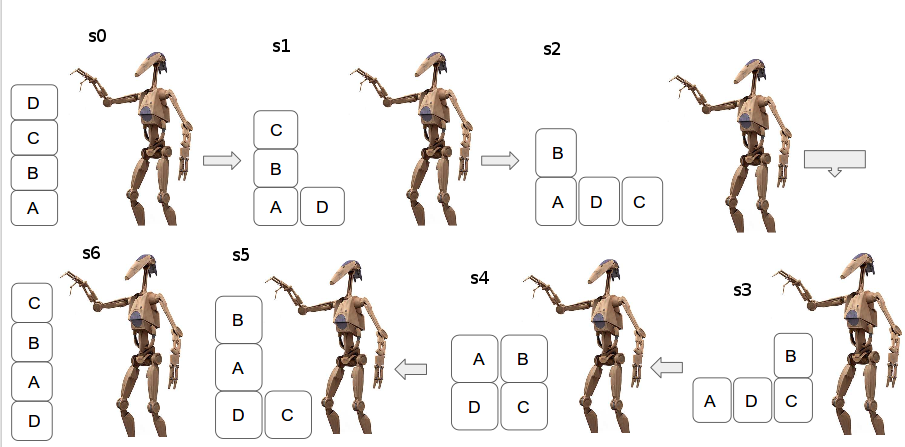
\includegraphics[scale=0.3]{StateTransitionEdit.png}
    \caption{Example of state transition, from one to another}
    \label{fig:StateTransition}
\end{figure}
In Figure \ref{fig:StateTransition} we have 7 states in total ranging from $s_0, s_1, s_2, s_3, s_4, s_5, s_6$. After an action has been performed it leads us to the next state. Now we can put the classical planning definition into some perspective, for example, we have 4 blocks, labelled A, B, C and D. A robot R1, an initial state onTable(A, B) onTable(C, D) meaning that all 4 blocks are placed on a table, and a simple goal state of on(A, B) on(C, D) meaning that we need to stack $(A\wedge B)$ and $(C\wedge D)$. This is a simplistic way of explaining the methods involved in planning and how a planner would solve this problem. What a person would do is assess the quickest and most efficient way (to them) to solve. Taking block A and putting it on top of B, and the same for block C and block D. A planner (depending on the algorithm) will create a type of search tree and explore each state by generating successors of already-explored states.
\begin{figure}[!htb]
    \centering
    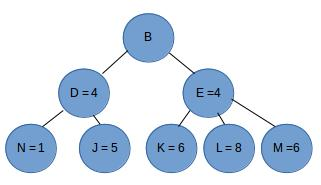
\includegraphics[scale=2.0,width=0.70\textwidth]{TreeExample.jpg}
    \caption{Basic example of a search tree with starting node B and goal node N\cite{PlanningBook}}
    \label{fig:Tree Example}
\end{figure}

As you can see in Figure \ref{fig:Tree Example}, if the goal was to find the shortest path from an initial state B to a goal state N, the planning algorithm would expand D and E, and from this would assess that N is a child of D. The algorithm would quickly find the node N in the tree graph and the cost for getting from B to N would be 5. 
\section{The Goal}
The goal for this thesis is to evaluate and test the techniques used in the PDDL4J library. In my opinion, the range of algorithms that can be used for planning is very wide and the current approaches are not optimal.  
In the following sections we will discuss the types of technologies that will be used throughout this thesis. We will start with the PDDL language in which domains and problems are encoded, then I will speak briefly about the PDDL4J library, introduce heuristics and finish with satisfiability problems.
\section{PDDL}
With the basics on planning covered, we can see how it is incorporated into the PDDL (Planning Domain Description Language), which is the main language for classical planning problems and domains. PDDL is used to express what predicates there are, what actions are possible, action structures and what the effects of those actions would be.\cite{PDDL1.2} Each type of problem for example, 'Blocksworld' or 'Mystery', will have a number of problems ranging from easy to hard, as well as a domain. The domain will provide the actions of what can be done, for example picking up a block as in Figure \ref{fig:StateTransition}. The problem file will begin with the objects that tell the planner how many items there are, such as 'objects: A B C D - blocks'; the more objects, the harder the problem. It will also define an initial state which will let the planner know what state the blocks are in, for example '(onTable B)', and will provide a goal state which the planner must satisfy. 
The main components of the PDDL represented as a planning task are:
\begin{itemize}
\item Objects = The blocks in this case (A, B, C, D)
\item Predicates = Properties of objects – these can be true or false. For example: Is A a block?  
\item  Initial state and goal state = The starting state of the world and the goal state of the world. All blocks are on the table and the goal is for them to be stacked in a specific order.
\item Operators/Actions = The actions that can be used to complete the task, broken down into preconditions and effects. Each precondition and effect can be positive or negative. \ldots
\end{itemize}
Each of the above are split between the domain file and the problem file. The domain handles the predicates and actions while the problem handles the initial state, goal state and the objects. 

If we look at the domain we can see the schema for the Blocksworld problem (see Figure \ref{fig:Blocksworld Domain} below). Inside we have some requirements at the top which tells the planner if it's able to solve the problem. It does this by informing the planner of the types of actions it will find within the domain, conditional effects, equality etc. As PDDL is a huge language, there are multiple subsets that have been created because very few planners would be able to incorporate all versions of the PDDL language. 
\begin{figure}[!htb]
    \centering
    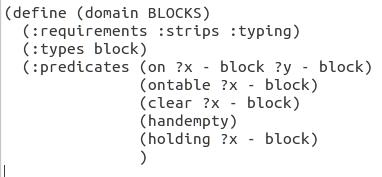
\includegraphics[scale=1.8,width=0.70\textwidth]{BlocksworldDomain1.jpg}
    \caption{Example of domain schema from Blocksworld domain}
    \label{fig:Blocksworld Domain}
\end{figure}
Next the actions associated with that domain will be specified. The actions will reflect the requirements (Figure \ref{fig:Blocksworld Pick-up Action}) and the planner will use these actions to help it solve the problem. 
\begin{figure}[h]
    \centering
    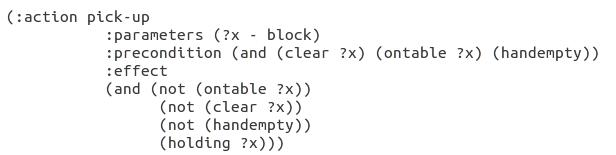
\includegraphics[scale=2.0,width=0.70\textwidth]{BlocksworldDomainAction.jpg}
    \caption{Example of an action pick-up from Blocksworld domain}
    \label{fig:Blocksworld Pick-up Action}
\end{figure}
\\
\\
The action in Figure \ref{fig:Blocksworld Pick-up Action} is a pick-up action; it tells the planner that it can only pick up one block at one time and, when it is picked up, it is at location x. An action can only be executed when the preconditions of that action are fulfilled; when the execution takes place, this generates effects, i.e. changes within the environment, for example:
\begin{itemize}
\item Block A has been picked up = Action
\item Clear A must be true before the robot can pick it up, therefore, nothing can be on top of block A = Precondition of the action PickUp
\item The negative effect of this action is that the Block A is now not on the table and the robot's hand is not empty. The positive effect of this action is that the robot is now holding Block A = Negative/Positive effects 
\end{itemize}

The planner will use actions like these, and others that are coded in a similar fashion, to complete a problem. Below is a problem example which shows the objects (in this case 4), the initial problem stating the blocks that are clear, the blocks that are on the table and that the robot's hand is empty, and then finally the goal state. 
%INPUT PROBLEM PHOTO HERE
\begin{figure}[!htb]
    \centering
    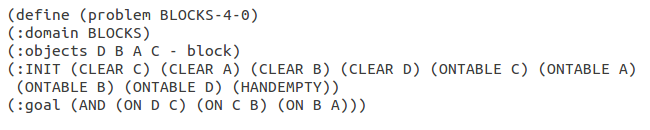
\includegraphics[scale=2.0,width=0.70\textwidth]{BlocksworldProblem.png}
    \caption{Example of a problem from Blocksworld 
    domain}
    \label{fig:Blocksworld Problem}
\end{figure}
\\
To tie all of the above together, the domain will provide the planner with the actions along with preconditions and effects for that action, and the problem will provide an initial state and a goal state that the planner must reach in order to satisfy the problem. 
\\
Now we can define a PDDL task by a 3-tuple $\Pi$ = ($S_0, G_n, O)$ where
\begin{itemize}
\item $S_0$ = Is a finite set of ground atoms called the initial state
\item $G_n$ = Is a closed formula called the goal formula
\item $O$ = Is a finite set of PDDL actions \cite{ConciseDomain} \ldots
\end{itemize} 

The initial state and goal state are the same as previously explained but, as the initial state begins at 0 and the goal state at \textit{n}, we are not sure where it is within the sequence. The axioms help us define predicates based on basic predicates. As seen by the example "given an \textit{ontop} predicate, we can define its transitive closure \textit{above} with the two axioms \textit{$above(x,y) \leftarrow ontop(x,y)$} and \textit{$above(x,z) \leftarrow \exists y(ontop(x,y)\wedge above(y,z))$}" \cite{ConciseDomain} With axioms like this, we ensure the evaluation is well defined and contains specific rules such as "ontable(A) is true when ontable(A) is actually false".   

\section{PDDL4J}

As discussed earlier, PDDL4J was created by Damien Pellier. The main components of the planner break down into three broad categories: 
\begin{itemize}
\item Preprocessing 
\item Search algorithm 
\item Heuristics
\end{itemize}
Using these three categories in unison creates a well-formed planner. The preprocessing side will take in all the facts from the domain of a PDDL problem and change each action condition using the variables, such as Block A, Block B etc. 
\begin{verbatim}
(:action pick-up
		:parameters (A - block) 
		:precondition (and (clear B)(ontable B)(handempty))
		:effect
		(and(not(ontable A)) 
\end{verbatim}
In each problem, the objects are known from the beginning, so the preprocessing side of the planner will instantiate each operator with all possibilities. As well as, this there are a number of steps that need to taken into account before the final representation is presented to the search algorithm and heuristic. When the domain and problem are encoded, logical simplification is performed to convert the problem to a bitset representation as the final outcome.
%Check new paragraph was inserted
\\
\\
There are a number of different planning algorithms that can be used to find a solution to a problem; the PDDL4J library uses an algorithm called A*. The main idea behind A* is that it searches through all possible paths to the goal to find the shortest path. It is an iterative algorithm and, after each iteration, it decides which of the nodes to expand of the partial plan it has already made until it reaches the goal and computes the fastest route. It does this by using the simple function
\textit{f(n)= g(n) + h(n)} \cite{MinimumCostPaths} where
\begin{itemize}
\item\textit{n} = the last node in the path
\item\textit{g(n)} = the cost of the path from the start to \textit{n}
\item\textit{h(n)} = the heuristic that estimates the cost from \textit{n} to the goal
\end{itemize}

The A* algorithm will use the function above and then try to find the best and less costly route. It does this by examining the vertex $n$ that has the lowest $f(n)$ score. For example, if the cost from getting from a starting node \textit{A} to a goal node \textit{D} had two routes, one giving a total cost of 4 and another 6, A* will always choose the route with minimal cost. But A* cannot work on its own to find a solution to a problem, it needs to use a heuristic to assist it and guide it to the goal.

The role of a heuristic is to help look for an answer to a particular problem. It does not tell the algorithm what to find but only how to look for a potential solution. Within the PDDL4J library and with the A* algorithm, each heuristic plays a different role when used to help find a solution but will provide the same basic level of help, which is estimating the distance to the goal. 
\\
\\
In the context of mathematics, the Manhattan distance is the distance between two points measured along axes at right angles\cite{ManhattanDistance}. It can be written as $|x_1 - x_2| + |y_1 - y_2|$ when we have two points $p_1$ at $(x_1, y_1)$ and $p_2$ at $(x_2, y_2)$. This type of function can be used with the A* algorithm in the form of a heuristic to find the shortest path from $p_1$ to $p_2$. If we translate that into a heuristic function in the Java programming language, it will look more like this:
\begin{verbatim}
int distance = Math.abs(x1 - x2) + Math.abs(y1 - y2);
\end{verbatim}

If we wanted to incorporate the function above with A*, we would create a small algorithm that would increase the value of \textit{g} by \textit{distance} and decrease \textit{h} by \textit{distance} as we move closer to the goal. So, regarding, the A* function \textit{f(n)}, the A* function should have the same value as the \textit{distance} function defined above. If the two match then we would say that this heuristic is "admissible". 

Within the world of heuristics, two definitions exist: "admissible" and "non admissible". What is an admissible heuristic? We can say a heuristic \textit{h} is admissible if $h(s) \leq h^*(s)$ for all states \textit{s}. In other words, when estimating the distance from a starting node to a goal node, it does not overestimate. Then for a non admissible heuristic, there is a possibility that it will overestimate or underestimate the distance. Within the PDDL4J library there are two admissible heuristics, $h^m$ and $h^{MAX}$, but these will be discussed later. 

\section{Satisfiability Problem}
In the previous subsections, we looked at PDDL and how it works. This section and one in Chapter \ref{Chapter2} dedicated to a set of problems termed satisfiability (SAT) problems. These are a set of expressions which are boolean, which means there are only two possible outcomes, i.e. either true or false. It is expressed in propositional logic and uses the operators AND(conjunction, $\wedge$), OR(disjunction, $\vee$) and NOT(negation, $\neg$). We say a problem is satisfiable if all the variables can be set to true or false. There is a particular structure that needs to be kept when working with satisfiability problems – we will look at the notation briefly. 
\begin{itemize}
\item A literal can be positive or negative – $p_1$ is positive and $\neg p_2$ is negative. 
\item A clause is a disjunction of literals.
\item A formula is in conjunctive normal form (CNF) if it is a conjunction of clauses.\cite{SurverySat}
\end{itemize}
As stated above, we have $p_1$ and $\neg p_2$. $p_1\vee \neg p_2$ is a clause and $(p_1\vee \neg p_2) \wedge (\neg p_1 \vee p_2 \wedge p_3) \wedge \neg p_1$ is a formula in conjunctive normal form. 
If we set $p_1$ = false, $p_2$ = false we get $(F \vee T) \wedge(T \vee F \vee p_3) \wedge T$ 
\\
($p_3$ is arbitrary which means it is not assigned a value)
\\
\\
Using CNF rules\cite{Conjunctive}, we can deduce the above formula as $T \wedge T \wedge T$ = True.
As this formula has been classed as true because of the rules applied in propositional logic, we begin to see how it can be useful in terms of planners and solving complex problems.
\chapter{Literature Review} % Main chapter title

\label{Chapter2} % For referencing the chapter elsewhere, use \ref{Chapter1} 

\section{All About Research}
Within this chapter we will discuss the research undergone that has helped to reach the conclusion of the overall hypothesis. This will be discussed later on in the chapter. The beginning will be a brief overview and foundation of research, followed by research papers grouped by ideas, a model of processes carried out and the hypothesis of this paper. 
\section{PDDL}
The research undergone for PDDL was based around the language as there are multiple versions that have been released over the years since it was first introduced in 1998 for the first IPC (International Planning Competition) competition\cite{1998IPC}.
\begin{itemize}
\item 1998: STRIPS and ADL
\item 2000: STRIPS and ADL subset
\item 2002: PDDL2.1 Numeric and temporal planning
\item 2004: PDDL2.2 Derived predicates and timed initial literals
\item 2006: PDDL3 Soft goals and trajectory constraints 
\end{itemize}

We have discussed STRIPS and ADL in Chapter \ref{Chapter1}; the next version of PDDL incorporated numeric and temporal planning which was broken down into two subsets, PDDL 2.1 level 2 was the introduction of numeric fluents and PDDL 2.1 level 3 which was level 2 plus action duration. 
Numeric fluents(actions) allows the addition of integers within the conditions of an action\cite{PDDL2.1}. If we need to compare these numeric fluents, it is only possible between other numeric fluents. The effects of an action can be changed in such a way as to incorporate an increase or decrease in these numeric values, for example: 

\begin{verbatim}
(:types bottle)
(:functions
	(amount ?b - bottle
	(capacity ?b - bottle)
		(fluent number))
(:action empty
	:parameters (?b1 ?b2 - bottle)
	:precondition (>= (capacity ?b1) (amount ?b2)
	:effect (and (change (amount ?b1) 0)
	change (amount ?b2)
	(+(amount ?b1)(amount ?b2))
\end{verbatim} 
With this problem we have two bottles and some liquid which we use as the numeric fluent. The goal is to take the liquid from the first bottle and pour it into the second bottle but only if the second bottle has the \textit{capacity} to hold the amount of water from the first bottle. We use the word \textit{change} to update the numeric fluent of each bottle. You can see that the effect of the change in contents from bottle 1 to bottle 2 will result in bottle 1 having the numeric fluent value of \textit{0} as there is no liquid left after the action \textit{empty} has completed. 

A temporal action can be seen as a durative action as a way of modelling the temporal properties of a planning domain\cite{PDDL2.1}. Durative actions can be broken down into discretised and continuous actions. One way it can be expressed is with \textit{duration}. Duration can be applied at the start of an action, in the middle of an action or at the end of an action, so it needs to be placed in the correct area in the domain and should read accordingly. 
\begin{verbatim}
:duration (= ?duration 10)
\end{verbatim}      
An example of the syntax is above and this shows that an action will cost a duration of 10 (could be seconds, minutes, hours etc). 
\\%Check NEW PARAGRAPH INSERTED
\\
The next version of PDDL, PDDL 2.2, was introduced by Stefan Edelkamp and Jorg Hoffman\cite{PDDL2.2}. They created the term \textit{derived predicates} meaning that the predicates do not get effected by the actions. So a set of derivation rules are used instead in the form of:
\\
\\
\textbf{IF}  $\varphi(\overline{x})$  \textbf{THEN}  $P(\overline{x})$\cite{AutomaticPlanning}
\\
\\
\textit{P} is the predicate that can be derived with the vector variable \textit{$\overline{x}$} so then instances of \textit{P} can be true or false. 

Timed initial literals are used to express a restricted form of externally derived events. In other words, at a certain time point in the plan, a fact will become true or false. These times are known to the planner from the beginning in the initial state. As PDDL is moving towards real life events and how to take into account events that do not start out being true but then change as time moves on, using timed initial literals gives that impression. Let's say we have a queue of customers waiting to pay for their shopping with one sales assistant working on a checkout. In the beginning, we have a group of people and one checkout operator. We can say that in the beginning, checkout operator >1 = false. But at some stage, another checkout operator arrives so there are two checkouts now open to serve the customers. Checkout operator >1 has now changed to true. 

PDDL 3 was released in 2006 and introduces the concept of strong and soft constraints on plan trajectories\cite{PDDL3}. The proposition of soft constraints and goals are not required to be completed by the planner to have a valid plan but are more of a desire. A strong constraint or goal requires the planner to satisfy these requirements for a plan to be valid. With regards to soft constraints, a planner should try to satisfy as many of these as possible as it gives better plan quality, however, for strong constraints, these must be met by the planner. The soft constraint aspect can carry a penalty for not satisfying one of these goals/constraints. In other words, when a planner starts to solve a problem in PDDL 3, it must check first for the soft goals/constraints and if not all of them are achievable then the planner must select the costliest subset of soft goals to complete in order to minimise the penalty. This can be extremely difficult as there may be multiple soft goals/constraints that carry different penalty weights and even more so if the planner has a time limit in which to solve the problem. 
There are many ways to express soft and hard goals/constraints but see below as an example:
\begin{verbatim}
(forall (?p - players)
	(preference ScoreGoal
		(sometime (at ?x Score)))
\end{verbatim} 
This could represent a football (soccer) problem where every player on the team must score a goal. This would enforce a penalty for the total number of players that did not score a goal during the plan. We can set this penalty at any cost for each player that did not score. For instance, a striker (forward player) not scoring would have a penalty of 5 because that is his role but a defender would have a penalty of 1 because that is not his role within a game of football.

Now we can look at state trajectories that could be set as soft or strong constraints in the Blocksworld problem.
\\
\\
"Each block should be picked up at least once" 
\begin{verbatim}
(forall (?b - block) (sometime(holding ?b)))
\end{verbatim}\cite{PDDL3} 
This can be set as a hard or soft constraint depending on the requirements of the problem. One way to complete this task for a planner could be to solve the problem with the required blocks by remembering which were used, then pick up the remaining blocks and put them back down after the hard goals/constraints have been satisfied. 

As it is extremely difficult for a planner to incorporate all of the PDDL, in each research paper they use what is called the benchmark for classical planning. This is the recommended set of problems that have been used at the IPC competitions over the past number of years\cite{ICAPS}. For this thesis, STRIPS and ADL have been the choice for testing algorithms and generating results. It will be IPC 1-8, each with 5 domains per ICP, as this will enable fair comparisons to previous work done with STRIPS and ADL to be carried out. 
\section{Classical Planning Algorithms}
In this section, we will discuss the two types of algorithms (forward and backward search) in terms of planning. In state-space planning, we have forward and backward search. In plan space planning we search through a space of partial plans to find a solution. SAT planning turns the problem into a propositional satisfiability problem and given to a SAT solver. Finally we have HTN (Hierarchical Task Network) which is more of an approach rather than a technique of planning, but for this thesis we will focus on state-space planning for classical planning representation. 
\subsection{State-Space Planning}
Within state-space algorithms for planning, the main focus is to create a subset of the state space termed the search space. We can break it down into 3 sub-categories, i.e. each node corresponds to a state of the world, each arc corresponds to a state transition and the current plan corresponds to the current path in the search space\cite{PlanningBook}. We then have three types of algorithm that we can implement for state-space planning: forward search, backward search and a combination of the two. We are able to search in a forward or backward way because of the preconditions and effects. 
\subsubsection{Forward Search}
Best First Search (BFS) is an algorithm that came to light in 2003. The algorithm was developed from the \textit{general search} algorithm described in the book 'Artificial Intelligence: A modern approach'. We can edit this general search algorithm to enforce a best first search algorithm by providing a knowledge area on the queueing function\cite{AModernApproach}. The knowledge gained from the queueing function allows us to determine the next node to be expanded. So the general search algorithm can be easily changed to incorporate a knowledge-type function which evaluates nodes, and the node with the best evaluation is expanded first. 
Once we have the BFS algorithm, we can then incorporate a heuristic function $h(n)$ which estimates the cost of the least expensive path from the state $n$ to the goal state. We use this heuristic function to help select the next node to expand but it is not always the best node overall. When we use a heuristic with BFS, it changes to Greedy Best First Search (GBFS). We consider the algorithm to be susceptible to false starts\cite{StochasticHillClimb}. As an example, say we have a starting node A and we must get to the goal node D. In a tree-like approach, the GBFS algorithm will look for a direct route to the goal and, instead of expanding the two children of A which are B and C, it will only expand one, which could lead the algorithm to a dead end. This means that the algorithm can get stuck and break or we need to introduce a method that will detect repeated states. So if the algorithm goes back to A, it does not go back to B, but instead expands C. 
Another example of how the algorithm works is shown below. In Figure \ref{fig:GBFSTree} the goal is to find the highest cost in the tree, i.e. expand the nodes and generate the highest score.
\\ 
\begin{figure}[!htb]
    \centering
    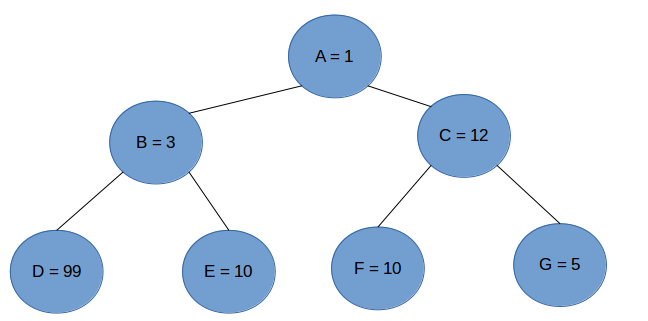
\includegraphics[scale=1.5,width=0.50\textwidth]{GBFSTree.png}
    \caption{GBFS algorithm trying to find the highest score from the nodes}
    \label{fig:GBFSTree}
\end{figure}
\\
The GBFS algorithm will work by selecting the nodes with the highest cost due to the goal that has been set. The algorithm will select \textit{node C} instead of \textit{node B} because 12 is higher than 3. It will then select \textit{node F} because 10 is higher than 5. The algorithm works in such a way that it will never reach the highest scoring node, \textit{node D}. As you can see it works by selecting the optimal immediate choice instead of expanding both nodes \textit{B and C} and checking the successor.
\\
\\
Using a forward search algorithm means that we will start the search from an initial state and use actions within the domain in a certain sequence until a goal state is reached. One of the most popular and well used algorithms that works in a forward search manor is A*. This is the current algorithm implemented in the PDDL4J planner. It was created in 1968 and is an extension to the Dijkstra algorithm\cite{MinimumCostPaths}. As well as being a forward searching algorithm, A* uses heuristics to guide its search towards the goal:

\begin{algorithm}
\caption{A*}
\begin{algorithmic}
\State $openList = set containing start$
\State $closedList = emptySet$
\State $start(g) = 0$
\While {$(openList \textbf{ is not } empty)$}
\State $current = openList(with lowest f cost)$
\If {$current = goal$} 
\State $constructPath(goal)$
\EndIf
\State $remove(current) \textbf{ from } openList$
\For {$eachNeighbour \in currentNeighbour$}
\If {$neighbour \textbf{ is not in } closedList$}
\State $add(neighbour)$
\Else { $openNeighbour = neighbour \in openList$}
\EndIf
\If {$neighbour = neighbour \in openList$}
\State $openNeighbour(g) = neighbour(g)$
\State $openNeighbour(parent) = neighbour(parent)$
\EndIf
\EndFor
\EndWhile
\end{algorithmic}
\end{algorithm}

We will look closely at this algorithm (see Algorithm 1 above) and the use of the weight functions $f(n) = g(n) + h(n)$. This essentially is the use of two types of algorithms, Best First Search and Dijkstra. If $h(n) = 0$ then $f(n)$ becomes $g(n)$ which is Dijkstra's shortest path algorithm. If $h(n) = \textit{large number}$ then $g(n)$ is ignored and it becomes Best First Search. So the use of an admissible heuristic with A* helps to balance out the two functions that make $f(n)$ which in turn creates a direct shortest path algorithm.\cite{InformedSearch}
From this we can see that A* is realistically more of a method than a point A to point B algorithm. Overall, it is a container for a greedy algorithm combined with a heuristic search function.  
\\
\\
Enforced Hill Climbing (EHC) is an algorithm that was implemented in a famous planner called Fast Forward (FF) \cite{FFPlanner}. EHC is an updated version of a generic hill-climbing algorithm. Hill climbing is used in mathematical optimisation in the area of local search. The main function in hill climbing is that it starts with an arbitrary solution and iteratively changes a single element in the original solution; if the new solution is better than the old then the old is replaced and the algorithm will continue to do this until no changes occur in the newest solution. 
Regarding EHC, what we want to achieve is a sequence of actions that in turn leads to a better successor if, at that moment, none are present. One of the main issues with EHC is that, with a heuristic to guide the search, EHC can get stuck in a dead-end or be unable to escape a plateau, meaning that within the search space, the heuristic values of all successors are greater than or equal to the best nodes already explored\cite{PlateauEHC}. What we would want to achieve when using EHC is to provide a method to escape the algorithm being stuck and never finding a solution within a specified time limit. 
\\ 
\begin{algorithm}
\caption{Enforced Hill Climbing}
\begin{algorithmic}
\State $openList = initialState$
\State $bestHeuristic = heuristicValue(initialState)$
\While {$(openList \textbf{ is not } empty)$}
\State $currentState = pop state \textbf{ from } head of openList$ 
\State $ successors = the list of states visible from currentState$ 
\While {$ successors \textbf{ is not } empty$}
\State $nextState = remove a state \textbf{ from } successors$
\State $h = heursticValue(nextState)$
\If {$nextState = goalState$}
\State $return(nextState)$
\EndIf
\If{$h is better than best heuristic$}
\State $clear(successors)$
\State $clear(openList)$
\State $bestHeuristic = h$
\EndIf
\State $place next state at back of open list$
\EndWhile
\EndWhile
\end{algorithmic}
\end{algorithm}
\\
In algorithm 2 above, we can see the comparison of the heuristic function $h$ and whether it is better than the best heuristic function available. 
\subsubsection{Backward Search}
A backward search algorithm does exactly what you would expect in that it works in the opposite way to a forward search algorithm by starting from a goal state and using actions in a certain sequence until an initial state is reached. 
There are many algorithms like A* and Dijkstra that can be used for forward search or backward search.
\\ 
\begin{algorithm}
\caption{DIJKSTRA}
\begin{algorithmic}
\State $dist[s] \leftarrow 0 $
\ForAll {$v \in V-(s)}$
\State $ dist[v] \leftarrow \infty$
\EndFor
\State $S \leftarrow 0$
\State $Q \leftarrow V$
\While {$Q \neq 0$}
\State $ u \leftarrow minDistance(Q, dist)$ 
\State $S \leftarrow S \cup (u)$
\ForAll {$v \in neighbours[u]$}
\If {$dist[v] > dist[u] + w(u, v)$}
\State $d[v] \leftarrow d[u] + w(u, v)$
\EndIf
\EndFor
\EndWhile
\State $return(dist)$
\end{algorithmic}
\end{algorithm}
\\
The distance to source is marked as 0 and we set all others to infinity. We then select the elements of $Q$ with the minimum distance and add $u$ to the list of visited vertices. Following this, we perform a check to see if a new shortest path can be found. If so, set the new shortest path value and return the distance. 
Dijkstra performed in a backward search will use the same approach and vertices with each arc $w(u, v)$ becomes $w(v, u)$ (see algorithm 3).
\section{SAT and SAT4J} 
SAT4J takes in files of CNF format as explained in Chapter \ref{Chapter1}. SAT4J is a Java library for solving boolean satisfiability and optimization problems\cite{SATandSAT4J}. It is able to solve a range of different types of problems and its written in Java. It is open source and uses a pseudo-boolean solver as a universal engine which translates the problems\cite{SATandSAT4J}. 

\begin{figure}[!htb]
    \centering
    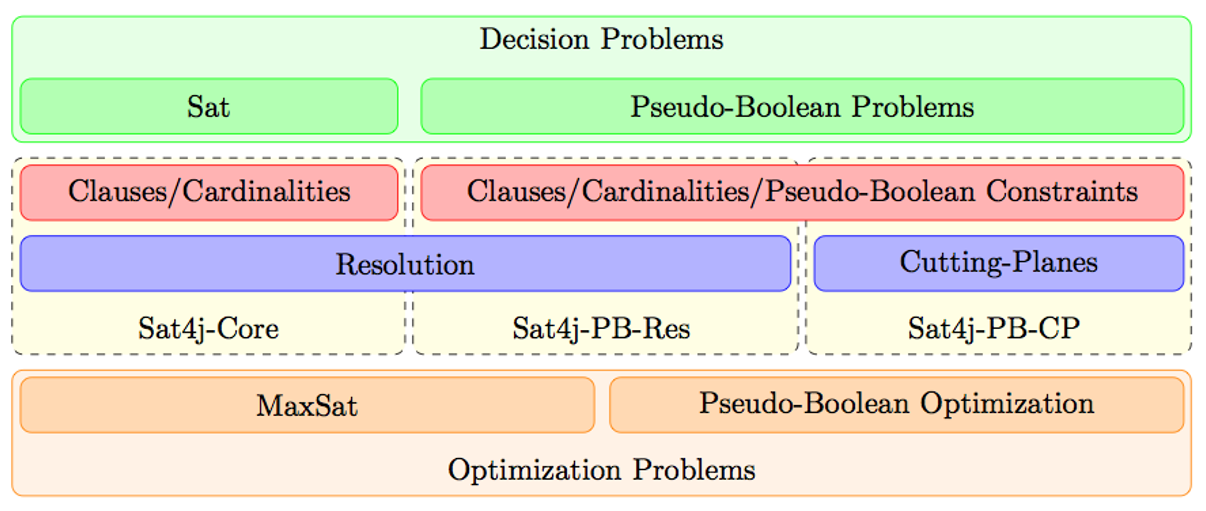
\includegraphics[scale=0.27]{SATFeaturesNew.png}
    \caption{Overview of the SAT4J features}
    \label{fig:SAT4J}
\end{figure}
In Figure \ref{fig:SAT4J} you can see an overview of the SAT4J system\cite{SATandSAT4J}. SAT was the first problem within the planning domain to be NP-complete based on the Stephen Cook theorem\cite{SteveCook}. NP represents for Non-deterministic Polynomial time and NP-complete means that any problem can be solved in polynomial time using a non-deterministic Turing machine. This is a theoretical concept in the field of computer science.
Below we show the basic semantic for a CNF file. 
If we have a formula:
\begin{verbatim}
(p(1) OR (NOT p(3)))
AND
(p(2) OR (p(3) OR (NOT p(1)))
\end{verbatim}
we can convert this into CNF format like so:
\begin{verbatim}
p cnf 3 2
1 -3 0
2 3 -1 0
\end{verbatim}
The first line \textit{p cnf 3 2} means that this is the first line of the problem; it is in conjunctive normal form; and there are 3 variables and 2 clauses. The next lines below are the clauses and they finish with a \textit{0} to let the solver know that the clause has finished. We represent \textit{OR} by a space in the clause and an \textit{AND} with a new line as seen above.
The SAT solver will then decide if this problem is satisfiable (or not) depending on the input by the user.
\begin{verbatim}
c 2 constraints processed
s SATISFIABLE
v -1 -2 -3 0
c Total wall clock time (in seconds) : 0.023 
\end{verbatim}
\textit{(The 0 at the end has been outputted to show the end of the clause)}
\\% CHECK PARAGRAPH
\\
We can see from the above output that the problem was satisfiable in a total time of 0.023 seconds. Translating it back to logic it looks like this:
\begin{verbatim}
(NOT p(1) OR p(2) OR p(3)
\end{verbatim} 
 
\section{Heuristics}
As discussed in Chapter \ref{Chapter1}, a heuristic function will involve a relaxed version of the problem. In some heuristics, the plan is to relax the problem so that a small subset of it can be solved so it makes it less computationally expensive to solve a problem. When the planning problem is relaxed, the deleted list of actions is ignored. These are the negative effects of an action.\cite{IgnoringDeleteLists} 
\begin{verbatim}
  (:action put-down
	     :precondition (holding ?x)
	     :effect
	     (and (not (holding ?x))
\end{verbatim} 
Taking a look at this example above shows how, within PDDL, the negative effect of an action is coded within the domain but, with heuristic functions, we ignore these notations of $and(not(xxxx)$ for negative effects as they provide no help to the state of the environment.
The area of heuristics can be broken down into 2 categories: admissible and not admissible. An admissible heuristic $h$ for all $s \in S: h(s) \leq h^*(s)$. This will mean that it does not overestimate the distance to the goal node. Not admissible heuristics can over-estimate or underestimate the distance to the goal node. 
In the PDDL4J library there are a number of heuristics that have already been implemented; the table below shows a list of heuristics and if there are admissible or not admissible.
\begin{center}
  \begin{tabular}{ | l | p{3cm} | l |}
    \hline
    \textbf{Heuristics} & \textbf{Method} & \textbf{Admissible/Not Admissible} \\ \hline
    Adjusted Sum & $sum(cost(pi)) + delta(S)$ & Not Admissible  \\ \hline
    Adjusted Sum 2 & $cost(S) + delta(S)$ & Not Admissible  \\ \hline
    Adjusted Sum 2M & $cost(S) + delta(S)$ with mutex& Not Admissible  \\ \hline
    Combo & $sumheuristic(S) + setlevel(S)$& Not Admissible  \\ \hline
    Fast Forward & Uses a relaxed graph to ignore negative effects & Not Admissible  \\ \hline
    Set Level & Return the level of the planning graph where all propositions of the goal are & Admissible \\ \hline
    Sum & Sum all the individual costs of each action &Not Admissible \\ \hline
    Sum Mutex & Sum heuristic where mutual exclusions are computed & Not Admissible \\ \hline
    Max & Calculates the most expensive atom & Admissible \\ 
    \hline
  \end{tabular}
\end{center}
As there are multiple heuristics implemented within the PDDL4J planer, I will explain briefly a not admissible heuristic Sum and how it can be changed with one line to make it the Max heuristic which is admissible. 
\subsection{Sum $H^+$}
This heuristic function is called $h_0(s)$, otherwise known as the sum algorithm.
\begin{equation}
\begin{aligned}
Delta(s)\\
  & \textbf{for each } p \textbf{ do}: if p \in s \textbf{ then } \triangle_0 (s,p) \leftarrow 0 \\
  & else \triangle_0 (s,p) \leftarrow \infty \\
  & U \leftarrow {s}\\
  & Iterate\\
  & \textbf{for each } a \textbf{ such that } \exists u \in U, precond(a) \subseteq u \textbf{do}\\
  & U \leftarrow {u} \cup effects^+(a)\\
  & \textbf{ for each } p \in effects^+(a) \textbf{ do}\\
  & \triangle_0 (s,p) \leftarrow min {\triangle_0 (s,p), cost(a) + \sum q \leq precond(a) \triangle_0 (s,q)}
\end{aligned}
\end{equation}
We set the costs of the propositions appearing in the initial state as 0 and the cost of the rest $\infty$. We then update the costs until a fixed point is reached. So if we have a planning problem and each action has a $cost(a)$, we can try to estimate the distance to a proposition $p$ or $g$. We do this by summing all the individual costs of each action.\cite{PlanningGraphs} If there is a solution to the problem, the sum algorithm will achieve it in polynomial time. Although it is a very informative heuristic, it is not admissible. 
\subsection{Max $H^1$}
Max is a popular heuristic but is not widely used in planning competitions because, for any given state, max calculates the most expensive atom in the state. It works by considering a relaxed version of the problem. 
The max algorithm is the same as the sum algorithm except for one line.\cite{PlanningBook} The \textit{for} loop for the positive effects changes to:
\begin{equation}
\triangle_1 (s,p) \leftarrow min{ \triangle_1 (s,p), 1 + max{\triangle_1 (s,q) | q \in precond(a)}}
\end{equation}
The max heuristic is not as informative as other heuristics as it computes the most costly sub-goals. 

\section{State of the Art}
The best way to view state of the art in state-space planning is the International Conference on Automated Planning and Scheduling, otherwise known as the International Planning Competition (IPC) \cite{ICAPS}. This competition is for planners to be tested against others on different domains and problems. The competition has been running since 1998 and uses different domains each time that are submitted by teams incorporating different levels of PDDL. For each of the conferences there have been new PDDL additions as discussed earlier. 
The competition breaks the planners down into sub-categories.
\begin{itemize}
\item Deterministic part 
\item Learning part
\item Probabilistic part
\end{itemize}
Within each of these sub-sections are domains and problems that correlate to a specific task as it is difficult for all planners to be able to participate in all events. In this thesis, the deterministic section will be the main focus. 
\subsection{Search Algorithms and Heuristics}
Looking at a number of planners that participated in the IPC competition over the past years, A* has been used various times as the main search algorithm but has been incorporated with other search algorithms to give a better overall search. A main algorithm used is one designed by Malte Helmert for the Fast Downward planner\cite{FastDownward}. It is based upon the FF (Fast Forward) planner that was designed by Jorg Hoffmann and Bernhard Nebel.\cite{FFPlanner} The FF planner won the IPC competition in 2000 and is based upon two functions: a search algorithm called Enforced Hill Climbing with a Best First Search as its "back-up" search function, and a heuristic function called Graphplan. Figure \ref{fig:FFplanner} shows the system architecture for the FF planner; the heuristic Graphplan is called at every state by the EHC algorithm and it is a forward search planner.
 
\begin{figure}[!htb]
    \centering
    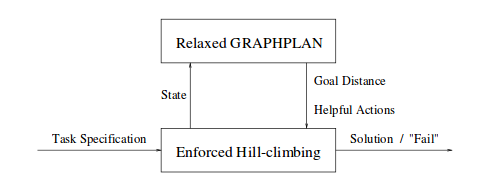
\includegraphics[scale=0.7]{FFplanner.png}
    \caption{System architecture for the FF planner}
    \label{fig:FFplanner}
\end{figure}

Fundamentally, it uses the EHC algorithm to find a solution to a problem but, as the algorithm is susceptible to getting stuck in dead ends as pointed out in \cite{FFPlanner}, there is a complete heuristic search engine built into FF that will start from the beginning if EHC fails, which helps to guarantee a solution. As well as the heuristic function, it has a backup algorithm Best First Search – and all of these functions together help build a very sound planner.  

Fast Downward is based on this approach and it was the winner of the IPC competition in 2004 \cite{IPC2004W}. It is constructed in the same way as FF as it is a heuristic search planner but it uses a different heuristic function called Casual Graph Heuristic. This heuristic approximates goal distances by solving a hierarchy of local planning problems \cite{CasualGraph}; these problems only include a single state variable and the dependant variable. Within a casual graph we think of nodes as the variables in the problem and the links within the graph show the dependencies among the variables. The estimate that it provides is the number of operators needed to reach the goal from a state $s$ in terms of estimated costs of changing the value of each variable $v$ that appears in the goal from its value $s(v)$ in $s$ to its value $s_*(v)$ in the goal.\cite{CasualGraph}
Malte Helmert and Hector Geffner describe the casual graph estimate function as:
\begin{equation}
h(s) = \sum_{v\in dom(s_*)} cost_v(s(v), s_*(v))
\end{equation}
The Fast Downward planner incorporates two actual search algorithms to create a plan. It uses a Greedy Best First Search (GBFS) with the casual graph heuristic, and the second is multi-heuristic BFS which combines different heuristic evaluators. The workings of the GBFS have been discussed earlier.
The multi-heuristic BFS works in a very simple way in that it will use multiple heuristics to direct the search towards a common goal. The idea behind it is that the heuristics will hopefully complement each other by having different weaknesses. So if one heuristic gets stuck in one section of the plan, the other heuristic may be able to find a solution for that particular problem efficiently and quickly and, therefore, negating the possibility of plateaus. But instead of combining the heuristic estimates into a single value, each heuristic alternates expanding a state from each open list.\cite{FastDownward}

Fast Downward uses a combination of a Casual Graph Heuristic and a Fast Forward heuristic (FF). The documentation for the Fast Downward planner \cite{FDownwardDoc} explains that both the Casual Graph heuristic and the FF are not admissible. From work previously carried out, a heuristic is not admissible when it may overestimate optimal costs.\cite{Pearl}\cite{Nilson} \cite{AdmissibleHeuristic} This shows that the Fast Downward planner in this sense is not optimal because it uses heuristics that are not admissible. Overall it means that when using these heuristics combined with the multi-heuristic BFS algorithm, the plans found are not optimal in terms of steps taken to achieve a goal. 
In the most recent IPC competition, the first-place planner in the deterministic track, the basis was Fast Downward and FF so we can see that using these algorithms provides non-optimal plans but this is sacrificed for speed and memory consumption, as well as solving problems. 

One of the main heuristics used by multiple planners is the Fast Forward heuristic, developed by Hoffmann and Nebel\cite{FFPlanningSystem}. Its main function is that from a current state, it finds a relaxed version of the problem and also ignores the negative effects from actions. The basis of the Fast Forward heuristic is that it uses a relaxed version of GraphPlan to compute the heuristic value. 

The algorithms over the years have not changed much but the heuristic functions have changed drastically. The PDDL4J planner has optimal heuristic functions that can be used with the A* search algorithm but A* is only an optimal search algorithm if the heuristic is admissible. 

From the two main planners we looked at in this section, the FF planner attempted 284 problems in the IPC 2002 competition and successfully completed 237 of them, giving it an 83\% success rate. The Arvanherd planner, the winner of the IPC 2014 competition, was built upon the Fast Downward planner and uses the FF heuristic. It was able to solve a total of 161 problems\cite{ArvandHerd}. The total success rate is unknown for Fast Downward.  
\section{Hypotheses}
In this section we will define the hypothesis for this thesis. Based within the PDDL4J library, there is reason to believe that the A* algorithm is not as optimal as other search algorithms. Yes, provided with the correct heuristic, it provides an optimal plan but is it optimal in terms of speed and memory consumption? Also, are the heuristics within the planner optimal in terms of plan size and are they truly admissible or not?

As stated in the previous section, there are other search algorithms and heuristics that provide fast and efficient results for classical planning problems. The goal is to implement a new search algorithm for the PDDL4J planner based on the research conducted and also a new heuristic. The PDDL4J library will be tested against the new algorithm and heuristic as well as tested against other planners from the IPC competition.

The last part of the thesis will show how a different area of planning can complete classical planning tasks. We will use the SAT4J library to run classical planning tasks and compare the results from the SAT4J library to the results from the PDDL4J library to see if satisfiability problems are easier to solve than classical planning approaches using PDDL.  
 
\chapter{Implementation and Methods} % Main chapter title

\label{Chapter3} % For referencing the chapter elsewhere, use \ref{Chapter1} 

\section{What to do with this research}
In this section we will discuss the methods that have been compiled for the literature review discussed in Chapter \ref{Chapter2} and how algorithms have been constructed. We will also detail the testing procedure for the new algorithms and how to assess the validity and reliability of these methods. In the final section will discuss the initial assumptions. 

\section{Algorithms and Design}
We will explore in detail the algorithms that will be implemented for the PDDL4J library and how the research brought us to the conclusion that these algorithms are more efficient than the existing ones. The search algorithm and heuristic have been taken from previous work in the classical planning field and applied to the PDDL4J planner.

As the PDDL4J library is written in Java, the best way to implement the new algorithms is to use the existing parser and lexer for the library and then remove all existing code for the A* algorithm and implement the new GBFS and EHC at the top level. As creating the parser and lexer would be a lot of work, we felt this was the better option as the existing code was efficient at parsing the domain and problem files. 

The two search algorithms were available in pseudo-code which made the implementation a lot easier. The enforced hill climbing has been used multiple times so information regarding it was widely available\cite{HeuristicDomain}. The two new algorithms will be broken down into the following sub-sections and evaluated. 
\subsection{Greedy Best First Search with Enforced Hill Climbing}
From the research conducted on search algorithms, we have made the decision to implement Enforced Hill Climbing (EHC) which was used in the Fast Forward planner \cite{FFPlanner} but instead of using A* or a modified version of it, we have decided to use a generic Greedy Best First Search algorithm\cite{AModernApproach}. The main reason for implementing EHC is due to its success at previous IPC competitions as well as being able to be implemented alongside another search algorithm like GBFS. We felt that it would improve the PDDL4J library in terms of speed, memory and solving problems.
As GBFS expands the node that appears closest to the goal and uses the function $f(n) = h(n)$. This means that it only uses the heuristic to guide the search. So if we incorporate GBFS as a back-up algorithm for EHC with the Fast Forward heuristic, this will make a faster/more memory efficient planner than A* with the Fast Forward heuristic which is what is used within the library at present. 
From the work carried out by Blai Bonet and Hector Geffner, they proposed changing an old planner HSP \cite{HeuristicNewResults} from a hill climbing algorithm to a Best First Search algorithm, and the results showed that there was a dramatic increase in the number of solved problems compared to just using EHC \cite{PlanningHeuristic}. One reason we want to combine these two algorithms is that the EHC algorithm is not complete and it has a problem with potentially getting stuck in infinite loops so we want to include GBFS as well as a relaxed heuristic like Fast Forward. 
Another main driving point why we think that A* can be beaten in terms of speed/memory consumption is that, in previous research, it states that A* is slower than other searching algorithms due to the computation of $h(s)$ for every new state, which is computationally expensive\cite{HeuristicNewResults}, therefore, we want to avoid this computation if possible. The decision was then made to incorporate the EHC and GBFS together to create potentially a fast, memory conscious planner that would rival A*.  

We have already introduced the EHC in Chapter \ref{Chapter2} as well as talked a little about GBFS but now we will describe how these two algorithms will work in depth and how they can complement each other. 
The use of a GBFS means that we will greedily expand the first successor that is found with a better heuristic value than its parent. But the algorithm will keep the parent stored so that the remaining children can be evaluated later. This, in turn, means that when we generate a successor state, two things can happen:
 
\begin{enumerate}
\item if the heuristic value of a successor is better than the parent, the parent is placed behind the successor in the search queue; or
\item if the heuristic value is not better than the parent, we use the value of the successor to place it in a priority queue and we continue the search.  
\end{enumerate}

In algorithm 4, we can see the pseudo-code for the GBFS algorithm. The aim is to perform heuristic evaluations that will be low as we envisage fewer successors.\cite{GreedyOnline}

An advantage in GBFS is that it can be a forward or backward search algorithm. In this case we will use it as a forward search and it falls into the category \textit{state space algorithm}, i.e. it looks through the space of possible states instead of looking for partial plans. With the implementation of these two new algorithms I purposed that the use of the Fast Forward heuristic that has been built within the PDDL4J library will be able to solve more problems than A* with Fast Forward and in faster times, as well as use less memory.
 
\begin{algorithm}
\caption{Greedy Best First Search}
\begin{algorithmic}
\State state = initialState 
\State h = initialHeuristic
\While {searchQueue \textbf{is not } empty}
\State currentQuery = pop item from front of searchQueue
\State currentState = state from currentQuery
\State currentHeuristic = heuristic from currentQueue
\State applicableActions = array of actions applicable in currentState
\ForAll{index $\in$ applicableActions $\geq$ counter}
\State currentAction = applicableActions
\State successorState = currentState.apply(currentAction)
\If {successorState = goal}
\State return(plan)
\EndIf
\State successorHeuristic = heuristicValue(successorState)
\If {successorHeuristic < currentHeuristic}
\State inset(currentState, currentHeuristic) 
\State insert(successorState, successorHeuristic)
\Else { insert(successorState, successorHeuristic}
\EndIf
\EndFor
\EndWhile
\end{algorithmic}
\end{algorithm}
\clearpage
\subsection{$H^m$ Heuristic} 
Here we will define the $H^m$ heuristic that was developed by Patrik Haslum and Hector Geffner\cite{AdmissibleHeuristic}. The $H^m$ heuristic is a domain-independent admissible heuristic which can be used to create optimal plans. This heuristic is part of the family of heuristics discussed in \ref{Chapter2} where we change a small section of the Max heuristic to create the $H^m$ heuristic. 
The new heuristic is based on computing admissible estimates of the costs of achieving sets of atoms from the initial state\cite{AdmissibleHeuristic}. This means that when we have a set of these atoms of size 1, it is basically equivalent to the Max heuristic.
\begin{equation}
\begin{aligned}
& h^m(g,s) = 0 \textbf{ if } g \subseteq s\\
& h^m(g,s) = \infty \textbf{ if } g \not\subseteq s
\end{aligned}
\end{equation}
The above equation is the beginning of the algorithm. It is stating that if the goal exists within the state $s$ then it is 0, and if it is not within the state then the node is unexplored so its set to infinity.
\begin{equation}
\begin{aligned}
& \textbf{if } |g| \leq k\\
& min_a (1 + \bigtriangleup^*(s, \lambda^{-1}(g,a)) | a\ relevant\ for\ g)\\
& \textbf{otherwise}\\
& max_{g'}(\bigtriangleup_k(s,g') | g'\subseteq g\ and\ |g'| = k
\end{aligned}
\end{equation} 
This was taken from \cite{PlanningBook} and it means that when $g$ has at most $k$ propositions, we take the exact value $\bigtriangleup^*$ but if that is not possible then we approximate the distance $\bigtriangleup_k$ to $g$. 
We then can break down this algorithm to give it more meaning – looking through \cite{PlanningBook} we see that $\lambda^{-1}(g,a)$ can be defined as:
\begin{equation}
\lambda^{-1}(g,a) = (g - effects^+(a) \cup precond(a)
\end{equation}  
Then further looking redefines $a$ to be relevant for $g$	 as:
\begin{equation} 
g \cap effects^+(a) \neq 0 \wedge g \cap effects^- = 0
\end{equation}
In\cite{PlanningBook}\cite{AdmissibleHeuristic} they both have recommended that the value of $k$ is kept at 2 because, as problems get harder with more objects, it is computationally expensive to generate subsets. The complexity of the heuristic makes the computation a polynomial $N^k$ where $N$ is the number of atoms. 
\section{How to Evaluate}
Based on a research paper by Carlos Linares Lopez, the new algorithms will be evaluated using the techniques discussed in \cite{Evaluation}. We will use all of the evaluation techniques as this will give a better idea of how effective the new algorithms are for the PDDL4J planner. 
The evaluation criteria is broken down into the following 4 categories:
\begin{itemize}
\item Objectivity – We want to have the same setting for all tests
\begin{itemize}
\item Representation Language – Keep the same order for each domain and problem as this can affect the outcome. Also the language used i.e. PDDL 
\item Evaluation Metric – Use one metric like time, plan size etc or if using multiple, keep it consistent throughout
\item Validation – Use a reliable system to validate the plans. It will ensure that the solution plans are logically sound 
\end{itemize}
\item Exhaustiveness – Use problems of a different nature, i.e. STRIPS and ADL, as well as multiple problem files within a domain which keeps the same problem structure but changes initial states and goal states
\item Comparability – Using well studied algorithms as a baseline for the new algorithms
\item Reproducibility – The test environment must be detailed so it can be replicated  
\end{itemize}
\subsection{How We Will Achieve This}
Within the domain of classical planning, the IPC competition has a number of domains and problems that are used each year to test the planners. So for the testing procedure, we have taken a number of domains and problems from each year of the IPC competition to make an extensive set of testing domains which will give a fair analysis of the new algorithms and methods. The tests will be run on a Linux server that has 24 CPUs, each Intel(R) Xeon(R) 2.30GHZ, as well as having 264.13GB of memory, which is more than capable of running the new algorithms. Each problem will be allowed 10 minutes to find a solution but if no solution is found within the time limit then the planner will skip and go on to the next problem. 

We will be using a piece of software called GNU parallel\cite{GNU} so the problems can be run sequentially to save time, however, the issue is that the threads that have been created to execute problems will be sharing resources so we need to try to limit the resources so that each thread has a specific amount. Below shows an example of one way we can use GNU parallel to test the program. The $seq$ allows us to start with the first problem and finish at the final problem (in this case 20). The $-j 6$ tells the server that we want 6 processes to be created and to run sequentially. The next part is allocating memory to each of the processes. We are opting for 8048 megabytes as we think this is a fair amount of memory for the planner. 
\begin{verbatim}
seq -w 20 | parallel -k -j6 java 
-javaagent:build/libs/pddl4j-3.1.0.
jar -server -Xms8048m -Xmx8048m 
fr.uga.pddl4j.planners.hsp.HSP -o 
pddl/benchmarks_STRIPS/ipc1/gripper/domain.pddl -f
pddl/benchmarks_STRIPS/ipc1/gripper/p{}.pddl 
-i 8 '>>' AstarGripper.txt
\end{verbatim}
There will be a variety of STRIPS and ADL problems within the tested domains. Each of the domains will have a range of problems from small to medium and hard. All of the actions within each domain will be listed in the same order, as well as the problem files. The domains that we will be testing are in the table below: the left column shows the domain name, the middle column shows the number of problems in each domain and the right column shows which IPC competition they are from. 
\begin{center}
  \begin{tabular}{ | l | c | r |}
    \hline
    \textbf{Domain} & \textbf{Number of Problems} & \textbf{IPC} \\ \hline
    Gripper & 20 & IPC1 \\ \hline
    Logistics & 30 & IPC1 \\ \hline
    Movie & 30 & IPC1 \\ \hline
    Mprime & 30 & IPC1 \\ \hline
    Mystery & 30 & IPC1 \\ \hline
    Blocksworld & 35 & IPC2 \\ \hline
    Elevator & 100 & IPC2 \\ \hline
    Freecell & 60 & IPC2 \\ \hline
    Schedule & 100 & IPC2 \\ \hline
    Depots & 22 & IPC3 \\ \hline
    Driverlog & 20 & IPC3 \\ \hline
    Rover & 20 & IPC3 \\ \hline
    Satellite & 20 & IPC3 \\ \hline
    Zenotravel & 20 & IPC3 \\ \hline
    Airport & 50 & IPC4 \\ \hline
    Optical Telegraph & 14 & IPC4 \\ \hline
    Philosophers & 29 & IPC4 \\ \hline
    Pipesworld & 50 & IPC4 \\ \hline
    Psr & 50 & IPC4 \\ \hline
    Openstacks & 30 & IPC5 \\ \hline
    Pathways & 30 & IPC5 \\ \hline
    Storage & 30 & IPC5 \\ \hline
    Tpp & 30 & IPC5 \\ \hline
    Truck & 30 & IPC5 \\ \hline
    Pegsol & 30 & IPC6 \\ \hline
    Sokoban & 30 & IPC6 \\ \hline
    Transport & 30 & IPC6 \\ \hline
    Barman & 20 & IPC7 \\ \hline
    Nomystery & 20 & IPC7 \\ \hline
    Parking & 20 & IPC7 \\ \hline
    Childsnack & 20 & IPC8 \\ \hline
    Hiking & 20 & IPC8 \\ \hline
    Thoughtful & 20 & IPC8 \\
    \hline
  \end{tabular}
\end{center}
The main test is the search algorithms, and they will be tested with the same procedure and the results will be compared in three areas:
\begin{itemize}
\item Time – How fast the planner can find a valid plan
\item Memory – What is the consumption of memory used to compute a valid plan
\item Plan size – What are the number of actions been completed to solve a problem 
\end{itemize}
Both search algorithms will use the heuristic Fast Forward and will be tested in the same environment. 
The new heuristic will be tested against three other heuristics: Max, Sum and Fast Forward. They will be tested using the same search algorithm (A*) and then compared in the same format as above but with one extra measurement, i.e. plan quality. This is where we look at each plan individually and assess when actions were executed to see if the admissibility of certain heuristics is true or false. Also, we will see how not admissible heuristics complete a plan and the steps they take compared to an admissible heuristic.
\subsection{Validity}
Validity is defined as \textit{"the quality of being logically or factually sound; soundness or cogency".} \cite{ValidityDef} In the context of this thesis, we will be using a plan-checking software that was used for the IPC 2002 competition\cite{ICAPS2002} which incorporates STRIPS and ADL (the use of which was decided in Chapter \ref{Chapter2} of this thesis). The plan-checking software was built for the competition by Stephen Cresswell and it works by generating parse trees for PDDL 2.1 syntax. It uses a range of different coding languages and functions to check if a plan is logically sound.
\textit{"A state-space planner provides a plan as a sequence of actions"}\cite{PlanningBook}. This is the goal for the new algorithms, i.e. to provide a sequence of actions that are logically sound, for example:
\\
\begin{figure}[!htb]
    \centering
    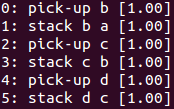
\includegraphics[scale=1]{SoundPlan.png}
    \caption{Example of a sound plan from Blocksworld}
    \label{fig:SoundPlan}
\end{figure}
\\
We can see from Figure \ref{fig:SoundPlan} above that there are no instances where the plan is incorrect. So at each step in the plan, the actions can be executed. An example of a non logically sound plan would be if, at step 2, the planner executed the action \textit{pick-up b}; this would not be possible unless the planner unstacked \textit{b} and \textit{a} first. 
\\
For validity we used a system called VAL which is a plan validator \cite{VAL}. It takes in a domain file, a problem file, a plan file, and tests to see if the plan is feasible given the set of actions in the domain and the problem.  
\section{Initial Assumptions}
The initial assumptions for the new search algorithm (GBFS with EHC using the Fast Forward heuristic) are that it will be able to provide a plan in a faster time and with less memory consumption than A* as well as being able to solve more problems from within the total amount. 
The new heuristic ($H^m$) will provide a critical path from starting node $s_0$ to a goal node $s_n$. In other words, the heuristic will sacrifice time and memory consumption but provide the optimal path. In comparison to other admissible heuristics where the plan length will be the same, we assume that the $H^m$ heuristic will complete different actions than other admissible heuristics in order to achieve a goal. 
\chapter{Evaluation} % Main chapter title

\label{Chapter4} % For referencing the chapter elsewhere, use \ref{Chapter1} 
\section{Before Testing}
In this Chapter we start the evaluation and testing procedure for the new search algorithm and heuristic. The first step is a preprocessing test, and when the results are analysed, we will start the preliminary tests of the new algorithms. 
\subsection{Preprocessing Test} 
The first thing to do before any tests could be completed was to check all of the IPC domains that would be used in the testing process for any errors. It would also give us a general idea of how long the parsing and encoding would take before the actual search could start. The goal was to remove any domains that had issues or that caused complications for the PDDL4J planner to encode. It would not make the testing environment fair if a domain was unable to be encoded properly and the search algorithm or heuristic ran for a long period of time when no solution would ever be potentially available. 
What we saw was issues with some of the domain files like Barman for example from IPC7. There were other domains like this and we addressed the issues and attempted to generate a new domain file or see if there was a small error inside the file that we could change.
\subsection{Preliminary Test}
In this section, preliminary tests were carried out to see if both the heuristic and the search algorithms were going down the right path to complete the hypothesis. We tested the search algorithm first by running it on the Blocksworld domain from the IPC2 competition. It was tested against the current A* algorithm and the preliminary results showed that the new search algorithms had out-performed A* by a considerable amount. The time for completing all 35 problems was much faster than A*, and also, A* was unable to complete the final 5 Blocksworld problems within the 600 second time limit. 

\begin{figure}[!htb]
    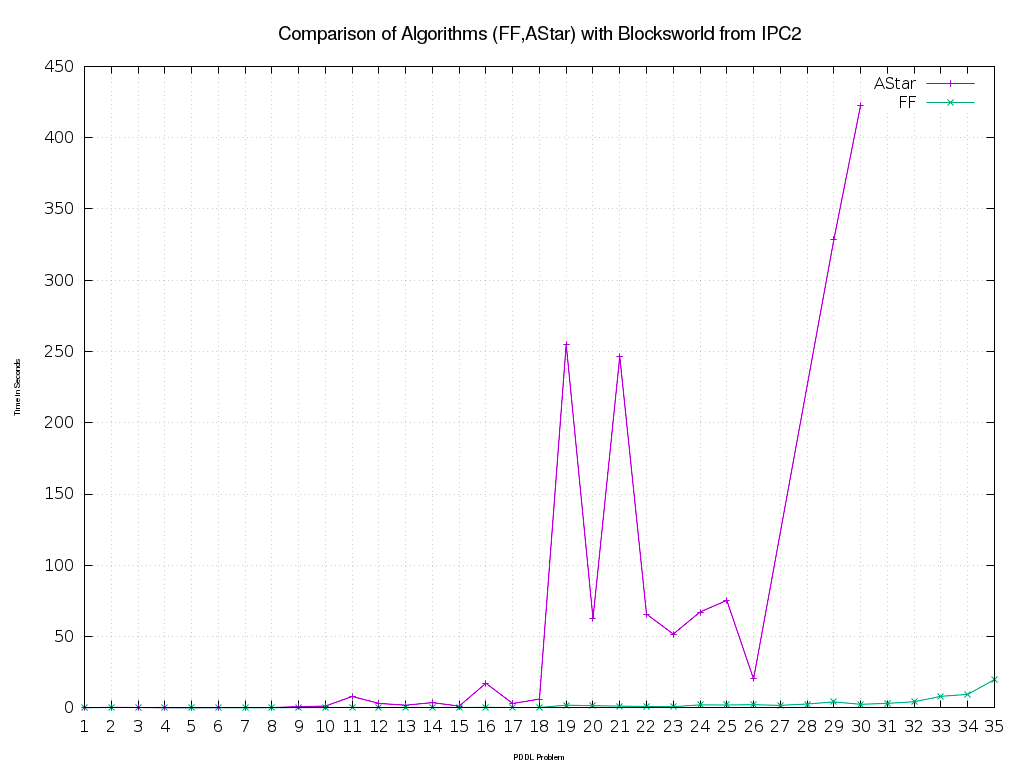
\includegraphics[scale=0.35]{PrelimTestFF.png}
    \caption{Preliminary results on the Blocksworld domain for the new search algorithm vs A*}
    \label{fig:PrelimVsA*}   
\end{figure}

This gave a really good insight to the capabilities of the new algorithm, as well as being on track to prove the hypotheses set out in Chapter \ref{Chapter2}. These results, however, could not be used as they were run on my own computer which does not fit in with the testing environment set out in Chapter \ref{Chapter3}.

The same environment was used to test the $H^m$ heuristic and it was tested on the Mystery domain from IPC1. We tested the new heuristic with Fast Forward and Max to compare the time needed to complete the problems. We achieved good results in that the new heuristic was similar in speed versus Fast Forward for completing the tasks although, as expected, the Max heuristic took longer. 

\begin{figure}[!htb]
    \centering
    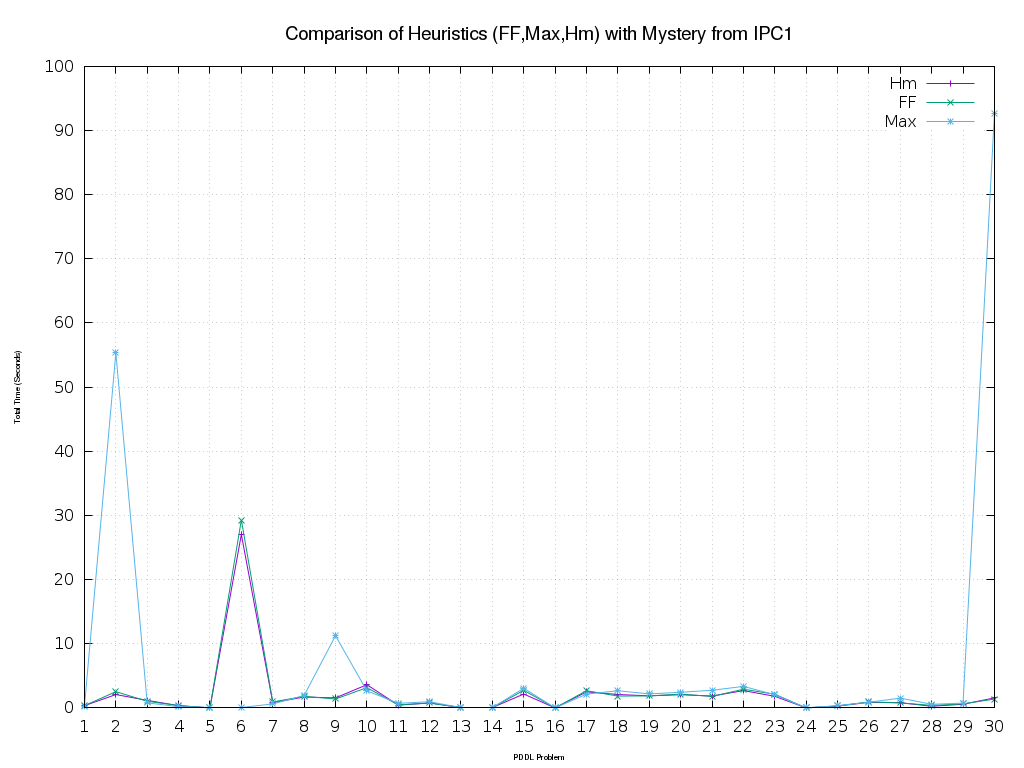
\includegraphics[scale=0.35]{PrelimTestHeuristic.png}
    \caption{Preliminary results on Mystery domain, FF vs Max vs $H^m$}
    \label{fig:PrelimFFvsMaxvsHm}
\end{figure}

There were no differences in plan size and we think this is because the $H^m$ heuristic is admissible \cite{hmAdmissible}, as is Max, so there should not be any differences in the plan length. Also, compared with Fast Forward, all plan lengths were the same. This is possibly due to the Mystery domain being a set of small problems with a small number of objects as well as all the heuristics running with the A* algorithm which should provide optimal plans (with the use of an admissible heuristic). A vigorous testing procedure in the next section should be able to provide the results that we are hoping for.  
\section{A* vs Greedy Best First Search and Enforced Hill Climbing}
As the preprocessing tests and preliminary results showed impressive data for the new search algorithm and heuristic, the testing stage can start against all domains from IPC1-IPC8 as discussed in Chapter \ref{Chapter3}
The table below shows all the domains in which we tested the new algorithm against A*. It also shows the total number of problems within each domain and how many of those problems the planners managed to solve. 
\begin{center}
  \begin{tabular}{ | l | c | r |}
    \hline
    \textbf{Domain} & \textbf{GBFS + EHC} & \textbf{A*} \\ \hline
    Gripper & 20/20 & 7/20 \\ \hline
    Logistics & 0/30 & 7/30 \\ \hline
    Movie & 30/30 & 30/30 \\ \hline
    Mprime & 14/30 & 24/30 \\ \hline
    Mystery & 13/30 & 16/30 \\ \hline
    Blocksworld & 35/35 & 30/35 \\ \hline
    Elevator & 99/99 & 99/99 \\ \hline
    Freecell & 60/60 & 59/60 \\ \hline
    Schedule & 0/100 & 0/100 \\ \hline
    Depots & 15/22 & 16/22 \\ \hline
    Driverlog & 16/20 & 14/20 \\ \hline
    Rover & 0/20 & 2/20 \\ \hline
    Satellite & 14/20 & 12/20 \\ \hline
    Zenotravel & 20/20 & 13/20 \\ \hline
    Airport & 0/50 & 28/50 \\ \hline
    Optical Telegraph & 1/14 & 2/14 \\ \hline
    Philosophers & 10/29 & 5/29 \\ \hline
    Pipesworld & 16/50 & 15/50 \\ \hline
    Psr & 41/50 & 47/50\\ \hline
    Openstacks & 30/30 & 7/30 \\ \hline
    Pathways & 7/30 & 5/30 \\ \hline
    Storage & 17/30 & 15/30 \\ \hline
    Tpp & 15/30 & 7/30 \\ \hline
    Truck & 13/30 & 8/30 \\ \hline
    Pegsol & 29/30 & 27/30 \\ \hline
    Sokoban & 25/30 & 25/30 \\ \hline
    Transport & 0/30 & 0/30 \\ \hline
    Barman & 0/20 & 0/20 \\ \hline
    Nomystery & 7/20 & 13/20 \\ \hline
    Parking & 3/20 & 0/20 \\ \hline
    Childsnack & 2/20 & 0/20 \\ \hline
    Hiking & 0/20 & 0/20 \\ \hline
    Thoughtful & 7/20 & 5/20 \\ \hline
    \textbf{Solved Problems Total} & 559/1089 & 538/1089 \\ \hline
    \textbf{Percentage} & 51.33\% & 49.40\% \\  
    \hline
  \end{tabular}
\end{center}
These are the results for the new algorithm for the PDDL4J planner versus A*. We used the same technique as described in Chapter \ref{Chapter3} to run the tests. A bash script was created so all the domains could be run one after the other and save the results in a text file which was then used to create diagrams with GNUPLOT. We can see some good results from the new search algorithm as well as some strange results, namely from the Rover domain where A* was able to solve only 2 problems out of a possible 20. Then with Airport from IPC4, A* was able to solve 28 out of a possible 50 but GBFS with EHC was unable to solve any of the problems. With Openstacks, GBFS with EHC was able to solve all 30 but A* could only manage 7.
The total number of problems in all of the domains is at the bottom of the table along with the total number of solved problems and the number of problems attempted against problems solved is shown as a percentage. From this we can deduce that GBFS with EHC was able to solve 1.93\% more problems than A*. Even though this is a small percentage, it is still an improvement in regards to the PDDL4J planner and it proves the hypothesis correct. We will now look at some of the problems in detail and explain the findings. All results for the tests are placed in Appendix A at the end of the report. 
\subsection{Graphs and Analysis}
There are many sets of domains that we could choose from but have narrowed it down to 4 in order to demonstrate the difference in time plus memory consumption between the two search algorithms. The domains are Movie from IPC1, Sokoban from IPC6, Blocksworld from IPC2 and Psr from IPC4. The full set will be displayed on GitHub and all information regarding access can be found in Appendix A.
\\
\begin{figure}[!htb]
    \centering
    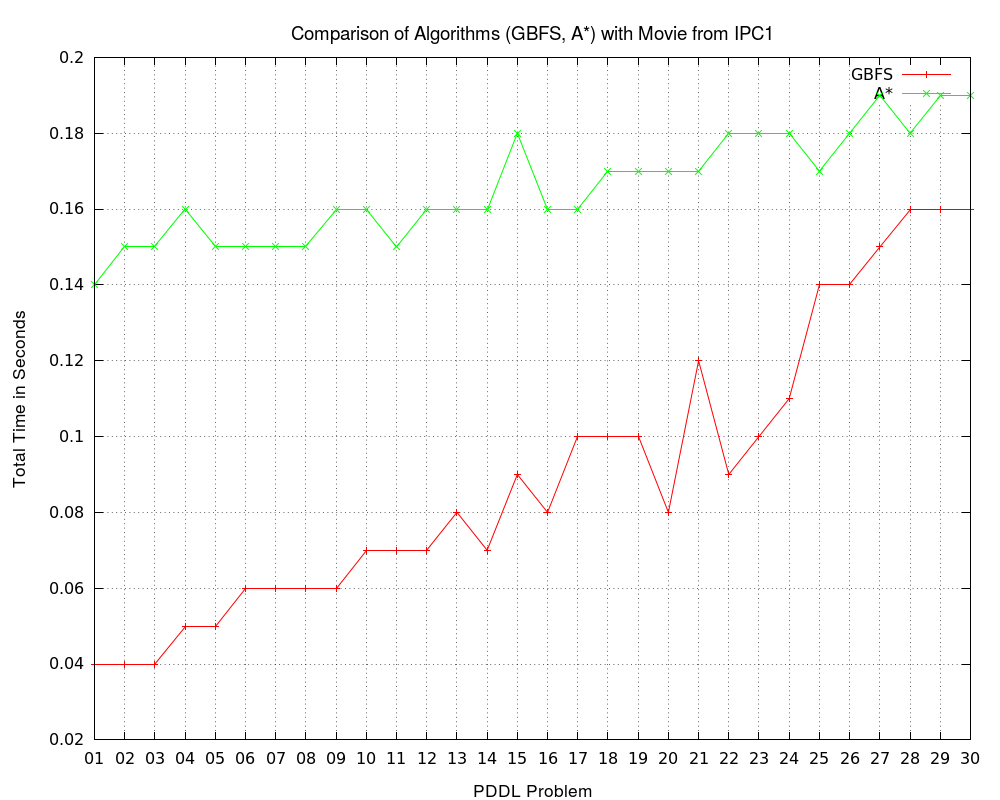
\includegraphics[scale=0.35]{MovieTime.png}
    \caption{Movie domain from IPC1, GBFS + EHC vs A* }
    \label{fig:MovieDomainTime}
\end{figure} 

The Movie domain has always the same goal, i.e. to get lots of snacks before watching the movie. The planners finish when all the snacks set out in the problem have been accumulated as well as the success of all other parameters set out in the problem. Each problem requires ADL, as discussed in Chapter \ref{Chapter2}. The problems for both planners are relatively easy but in terms of speed at achieving the goal, the new algorithm fairs better in every problem than A*. You can see from the graph (GBFS with EHC red, A* green) that the paths of the lines never cross or are even close to each other. Along the X axis is the time in seconds, the Y axis has the number of problems. We can see that the new algorithm as well as A* had a steady increase in line with the increase in difficulty of the problem and the time taken to solve them but even then, the times are not similar. From the raw data that can be accessed from the information in Appendix A, EHC failed for every problem but GBFS with EHC was still able to complete each problem faster than A*.
\\
\begin{figure}[!htb]
    \centering
    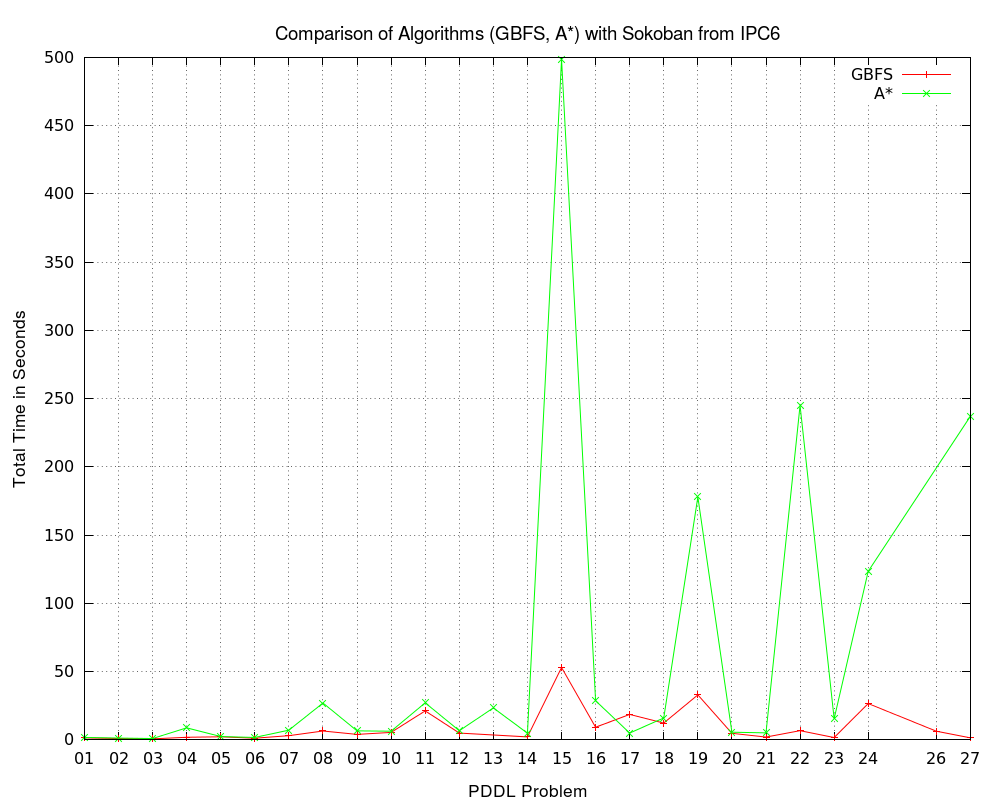
\includegraphics[scale=0.35]{SokobanTime.png}
    \caption{Sokoban domain from IPC6, GBFS + EHC vs A* }
    \label{fig:SokobanDomainTime}
\end{figure}
Let's look at the Sokoban domain which was used for the IPC6 competition. Sokoban is a game where there are crates in certain locations and the goal is to take one crate at time from the starting point to an end point but being careful not to block yourself in or get stuck. 
The domain has a total of 30 problems but both algorithms could only solve 25 each, however, the results regarding time are mostly better for GBFS with EHC.  From the graph it is clear that GBFS with EHC was able to solve the same number of problems but in a faster time; with some of the problems, the time taken is relatively close but in others there is a huge difference.    
\\
\begin{figure}[!htb]
    \centering
    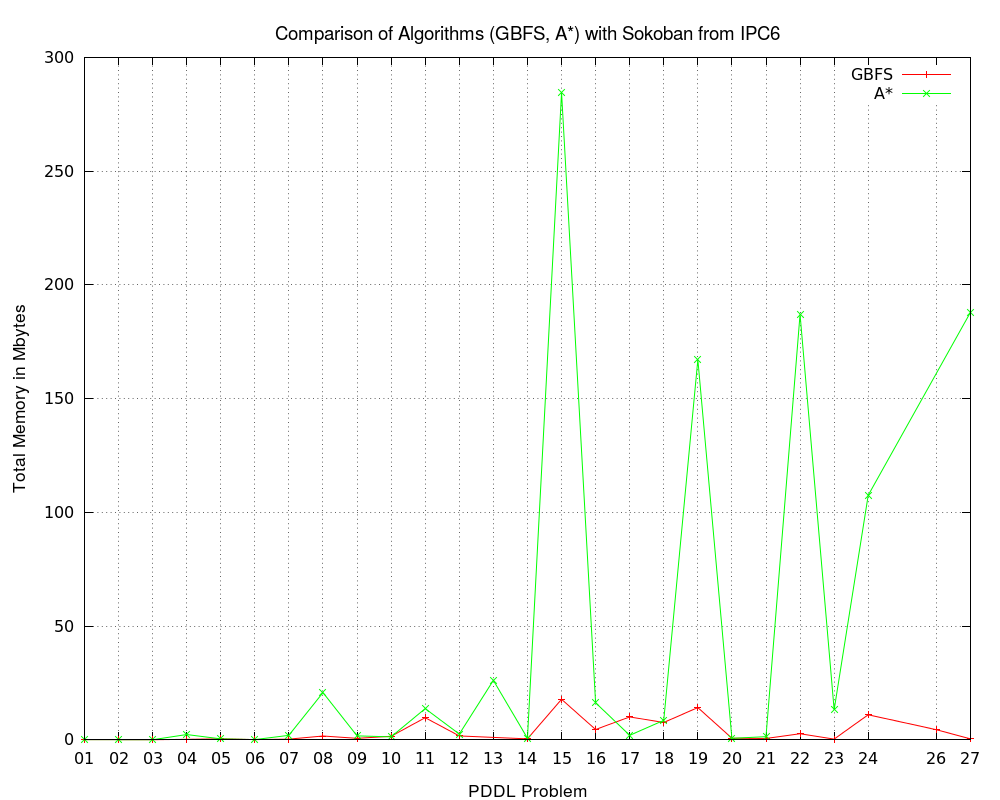
\includegraphics[scale=0.35]{SokobanMemory.png}
    \caption{Sokoban domain from IPC6, GBFS + EHC vs A* }
    \label{fig:SokobanDomainMemory}
\end{figure} 
Looking at the results on memory consumption for both A* and GBFS with EHC in the Sokoban domain, Figure \ref{fig:SokobanDomainMemory} shows that an increase in time yields an increase in memory consumption with the largest disparity showing up in problem 15. Here, GBFS with EHC was able to solve the problem in 52.99 seconds and use 17.82Mbytes of memory, whereas A* took 496.38 seconds and used 284.31 Mbytes, which is a difference of 443.39 seconds and 266.49Mbytes. To put this in perspective, GBFS with EHC would need to solve problem 15 in Sokoban 15 times in order to match the same memory consumption used by A*. 
Earlier in Chapter \ref{Chapter4}, we presented results of a preliminary test in the Blocksworld domain, showing the speed of GBFS with EHC.  Now, within the same domain, we will look at the memory usage for problems 01-35 (see Figure \ref{fig:BlocksworldDomainMemory}).
\\
\begin{figure}[!htb]
    \centering
    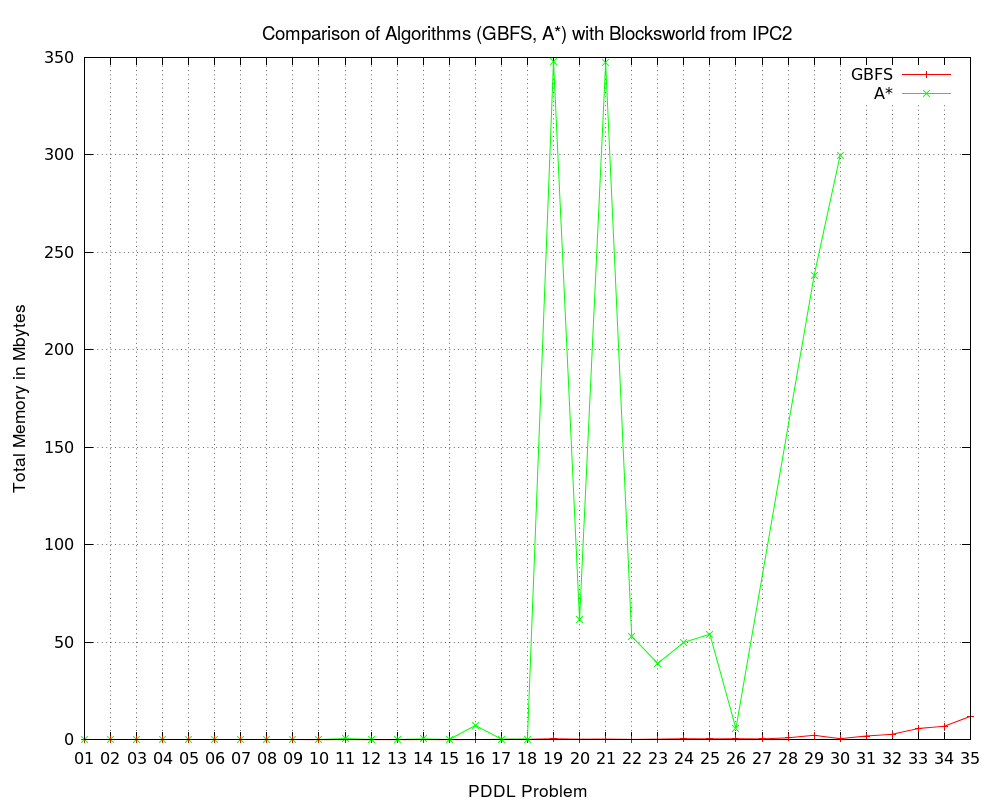
\includegraphics[scale=0.35]{BlocksworldMemory.png}
    \caption{Blocksworld domain from IPC2, GBFS + EHC vs A* }
    \label{fig:BlocksworldDomainMemory}
\end{figure}
From the graph we can see a very slow, steady increase in memory usage as the plans become more complicated for the GBFS with EHC algorithm, however, for the A* algorithm, things were more complicated. The maximum memory used by GBFS with EHC was done so when solving the hardest problem in the domain, i.e. 12.05Mbytes was used by GBFS with EHC for problem 35. If we look at the maximum memory used by A*, it was 348.12Mbytes and 347.07 Mbytes for problems 19 and 21 respectively, neither of which are the hardest problem. As well as this, we can also see that A* was unable to complete Blocksworld problems 31-35.
\begin{figure}[!htb]
    \centering
    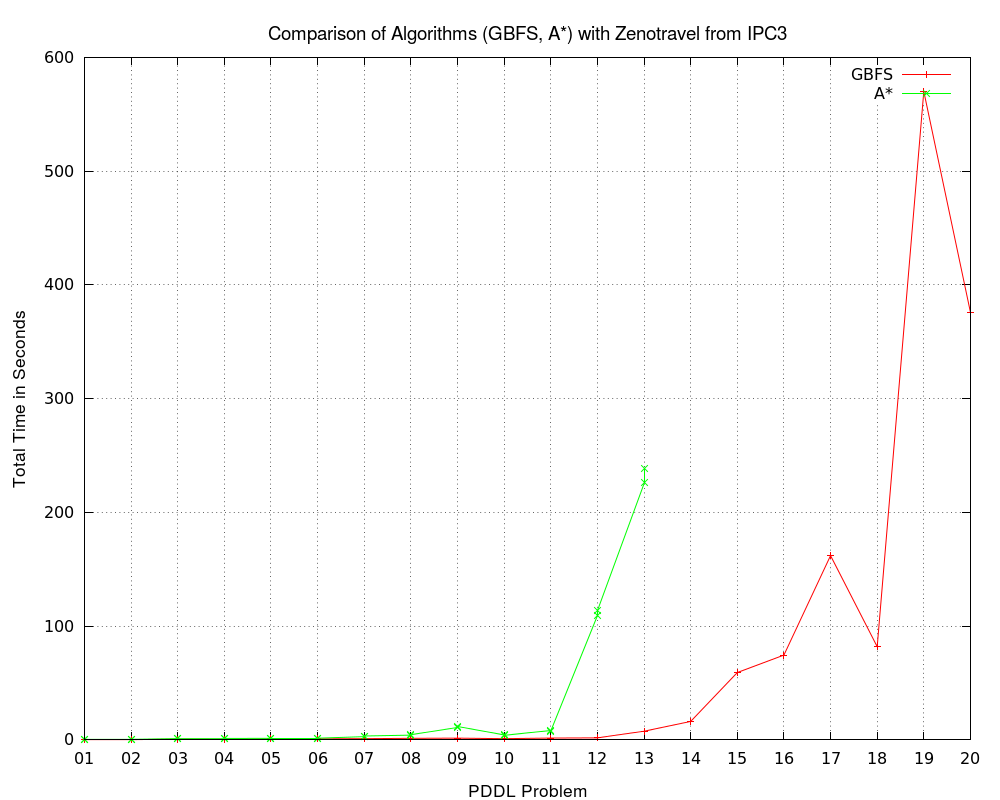
\includegraphics[scale=0.35]{ZenoTime.png}
    \caption{Zenotravel domain from IPC3, GBFS + EHC vs A* }
    \label{fig:ZenoTravelDomainTime}
\end{figure}
\\
If we look at Zenotravel from IPC3 Figure\ref{fig:ZenoTravelDomainTime}, GBFS with EHC was able to solve all 20 of the problems within the domain, but A* was only able to solve 13. The time gradually increases as the problems get harder in the domain for both algorithms but for GBFS with EHC there is a huge increase of time from problem 18 to 19. This could be because of the increase of facts, as problem 18 has 585 facts whilst problem 19 has 760. Also in problem 17 there is a total number of 16880 possible action which increases to 20970 in problem 18, then 19 has an even bigger increase to 26500. This increase could be the reason why the time has dramatically risen. 
\begin{figure}[!htb]
    \centering
    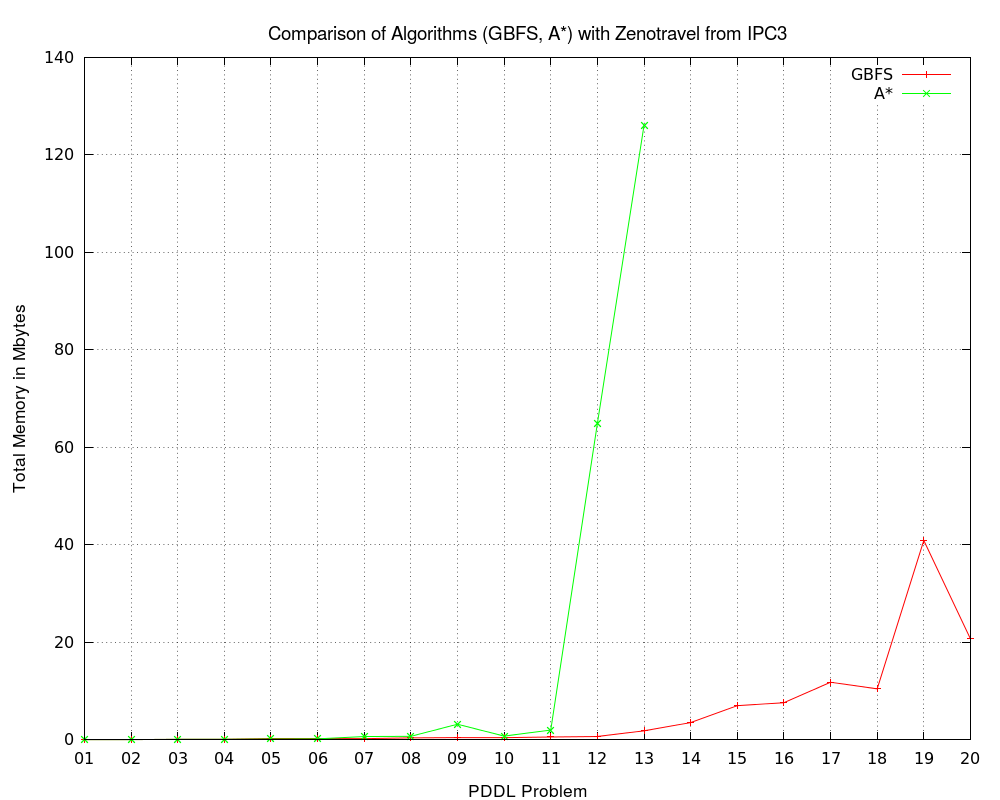
\includegraphics[scale=0.35]{ZenoMemory.png}
    \caption{Zenotravel domain from IPC3, GBFS + EHC vs A* }
    \label{fig:ZenoTravelDomainMemory}
\end{figure}
Then in contrast in Figure\ref{fig:ZenoTravelDomainMemory}, as the problems get harder, the memory consumption usually goes up along with it, which is what happened to A* but GBFS with EHC kept a steady increase of memory consumption with a small spike at problem 19. We can see by all the graphs shown that in terms of speed and memory consumption, GBFS with EHC is dominantly better.
\subsection{Null Plans}
Even though a preprocessing test was carried out for all domains, there were some that did not parse correctly and further analysing of these tests showed that some of the domains did not work correctly or there was issues with them which made it impossible for the planners to even attempt the domains. We can see automatically which domains or problems had potential problems as both of the planners were unable to solve any of the problems and the text files pertaining to the problem output were empty. To name one, the Barman domain was unable to be parsed correctly and that is why each of the algorithms have 0 solved problems.
\subsection{Validity}
As discussed in Chapter \ref{Chapter3}, we used VAL\cite{VAL} to check the new search algorithm to ensure that it was providing logically sound plans. As there were over 1000 tests, we selected a few problems to test using VAL. We felt that if these 5 tests came back positive then the algorithm was able to produce logically sound plans for all domains as we have a mix of STRIPS and ADL as well as easy, medium and hard problems. 
The 5 problems selected were:
\begin{itemize}
\item Problem 1 from PSR
\item Problem 10 from Zenotravel
\item Problem 20 from Blocksworld
\item Problem 01 from Sokoban
\item Problem 10 from Blocksworld
\end{itemize} 
All 5 of the tests came back positive and all 5 were valid. As there we no errors in any of the plans, we can assume that all plans will be valid from the new search algorithm.  
All raw data files can be found in Appendix B.
\section{$H^m$ vs Fast Forward vs Max vs Sum}
For comparison with regards to heuristics, we used the same search algorithm (A*) with all 4 of the heuristics. We tested them with the same script and same set of problems. As before, each problem was capped at 600 seconds to solve a problem. The results gained were not as good as the search algorithm and in terms of solved problems it was worse than expected. The $H^m$ heuristic was unable to solve more problems than any of the other 3 heuristics but we assumed this could happen as it is costly to generate all subsets of a problem. Because of this, the $H^m$ heuristic was only able to solve 12 of the Blocksworld problems within the 600-second time limit. The two admissible heuristics ($H^m$ and Max) performed worse in the Blocksworld domain. Max was only able to solve 6 more problems than $H^m$ but FF and Sum solved nearly all problems (see Figure \ref{BlocksworldDomainHeuristicCompare}). 
\begin{figure}[!htb]
    \centering
    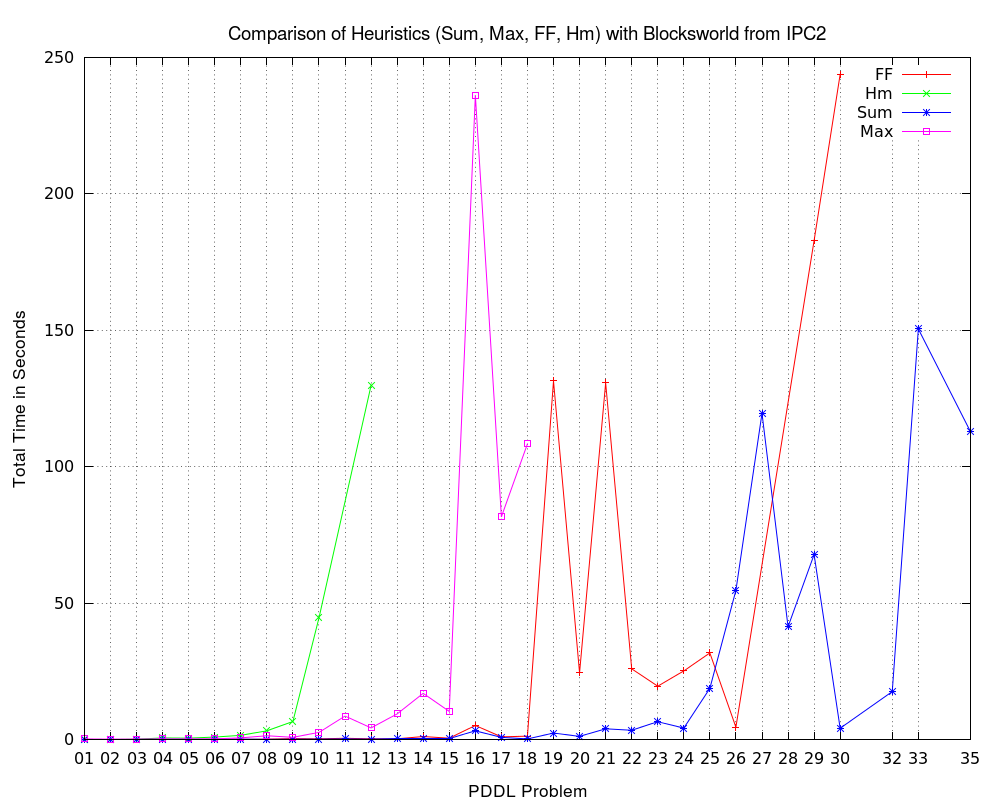
\includegraphics[scale=0.35]{BlocksworldTimeHeuristics.png}
    \caption{Blocksworld domain from IPC2, Sum vs FF vs Max vs $H^m$}
    \label{fig:BlocksworldDomainHeuristicCompare}
\end{figure}
If we then take a look at the Movie domain from IPC1 (see Figure \ref{fig:MovieTotalTimeHeuristics}, $H^m$ was able to solve all 30 problems, as could the other 3 heuristics. $H^m$ was a little slower than the other 3 in solving the problems but was able to do it within the 600-second time limit. Again, the not admissible heuristics proved to be better in terms of time within this domain. The memory consumption of each of the heuristics was exactly the same except for Sum being more efficient towards the end.
\begin{figure}[!htb]
    \centering
    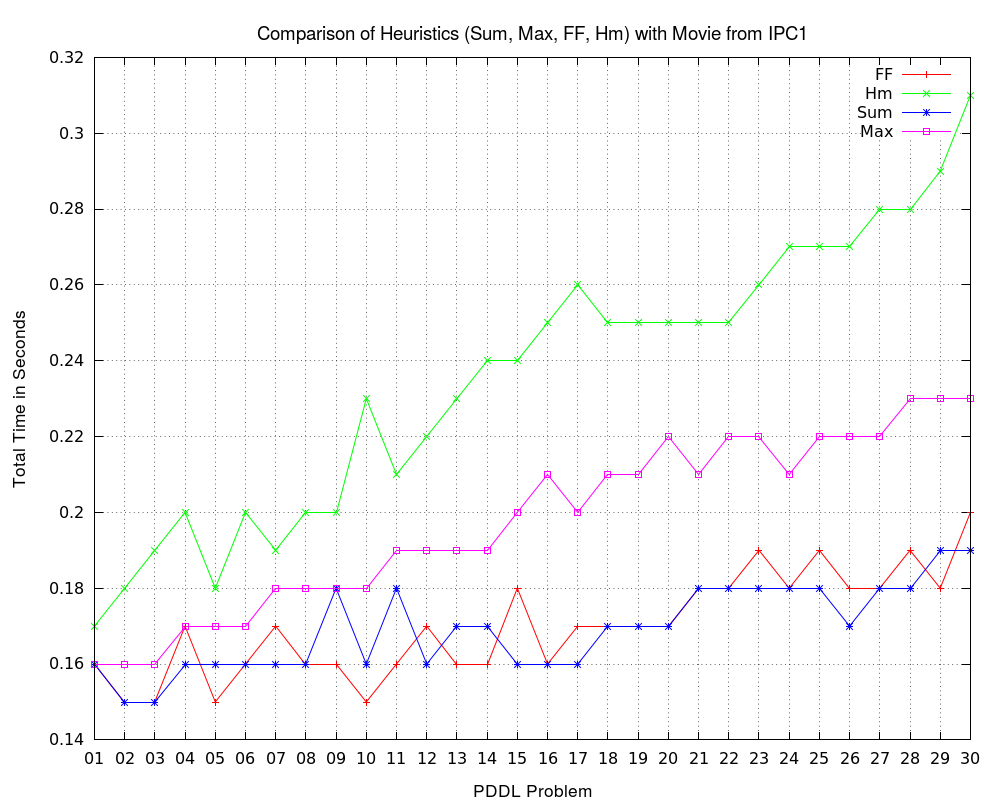
\includegraphics[scale=0.35]{MovieTotalTime.png}
    \caption{Movie domain from IPC1, Sum vs FF vs Max vs $H^m$}
    \label{fig:MovieTotalTimeHeuristics}
\end{figure}
The last strange result is that the plan size for all 4 heuristics was the same for each problem. Even though the Movie domain has many small problems, every problem having the same plan size for not admissible and admissible heuristics is not what we expected (see Figure \ref{fig:MoviePlanSize}). 
\begin{figure}[!htb]
    \centering
    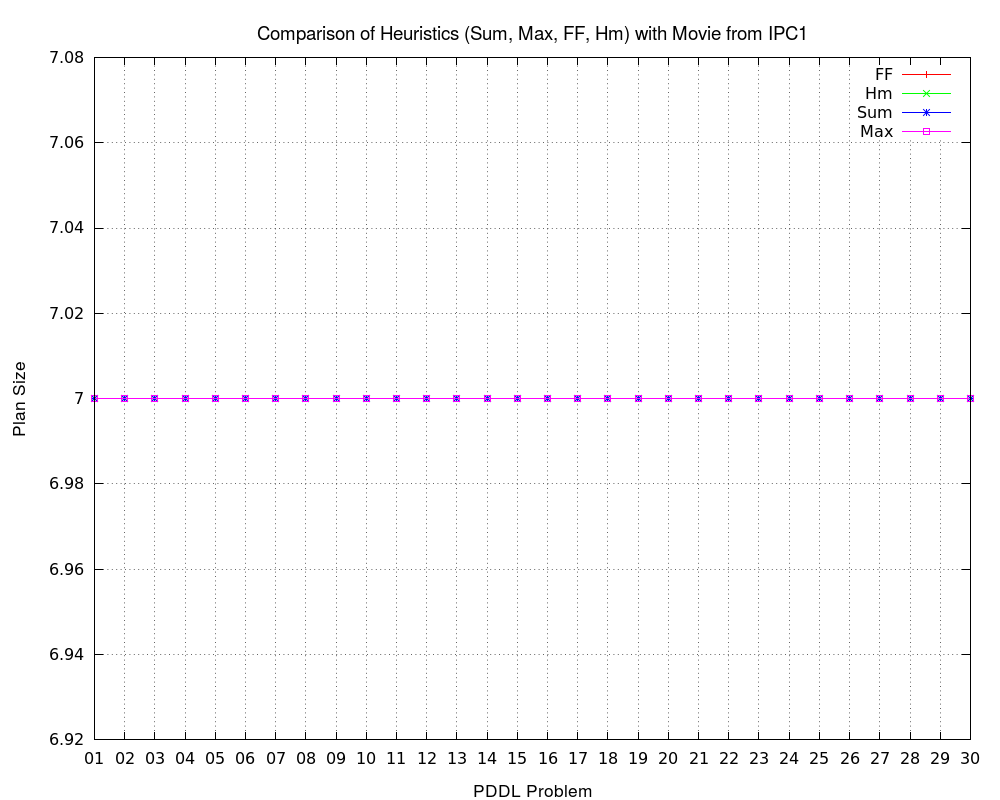
\includegraphics[scale=0.35]{MoviePlanSize.png}
    \caption{Movie domain from IPC1, Sum vs FF vs Max vs $H^m$}
    \label{fig:MoviePlanSize}
\end{figure}
As stated in \cite{HmHeuristic} the $H^m$ heuristic exhausts memory and this was the case multiple times during testing. Within a lot of the domains, the heuristic failed to solve any problems and memory was exhausted, that being said, within some of the domains compared to an admissible heuristic like Max, the results were similar in terms of solved problems but it was still the worse of the three. In some of the domains like Freecell, the $H^m$ heuristic was unable to solve any of the problems. 
What we saw was within the Blocksworld domain, there were anomalies between admissible and non admissible heuristic in terms of actions used to achieve a goal. 
%INSERT PICTURE!!!!!!!!
Above are the actions used to complete the Blocksworld problem 4 for all 4 heuristics. With regards to the two admissible heuristics $H^m$ and Max, we can see some differences in the actions used to complete the problem. At step \textit{02} the $H^m$ heuristic guided the algorithm to pick up block d whilst Max unstacked e b. Fast Forward and Sum did the same action at this stage. Even though all plan sizes are the same in length, these steps can describe a more critical path to the goal from the starting node. 
\section{SAT4J}
We wanted to test to see how a satisfiability planner solved PDDL problems. Even though there are a lot of SAT planners\cite{BlackBox}\cite{SATPLAN} we decided to take a Blocksworld problems and encode them to SAT problems within the PDDL4J library, then give the output to a SAT solver (in this case SAT4J) and see how much of a difference there was in terms of speed at solving satisfiability problems. We encoded 9 PDDL problems from the Blocksworld domain (p01-p09) and provided the files to SAT4J. 
We discovered that SAT4J was able to complete Blocksworld problem 9 within 0.037 seconds. Compared to A* which was 0.82 seconds and GBFS with EHC was 0.10 seconds. It shows that using a SAT solver is nearly 10x faster at solving problems. 
\begin{verbatim}
c org.sat4j.minisat.constraints.cnf.OriginalBinaryClause => 4
c org.sat4j.minisat.constraints.cnf.OriginalWLClause => 13
c ignored satisfied constraints => 17
c 34 constraints processed.
s SATISFIABLE
v -1 2 -3 -4 -5 -6 -7 -8 0
c Total wall clock time (in seconds) : 0.037
\end{verbatim}
Due to time constraints, only the Blocksworld domain was tested. With more time, we could test all of the IPC domains for a comparable analysis. 
\section{GBFS with $H^m$}
We combined the new search algorithm with the new heuristic to see if the plan size would be smaller when using a heuristic that should provide the optimal path. When the problems became harder, the GBFS with EHC + FF plan size grew but when applied with $H^m$, the plan size was considerably smaller as you can see from Figure \ref{fig:BlocksworldDomainGBFSwithHm}.
\begin{figure}[!htb]
    \centering
    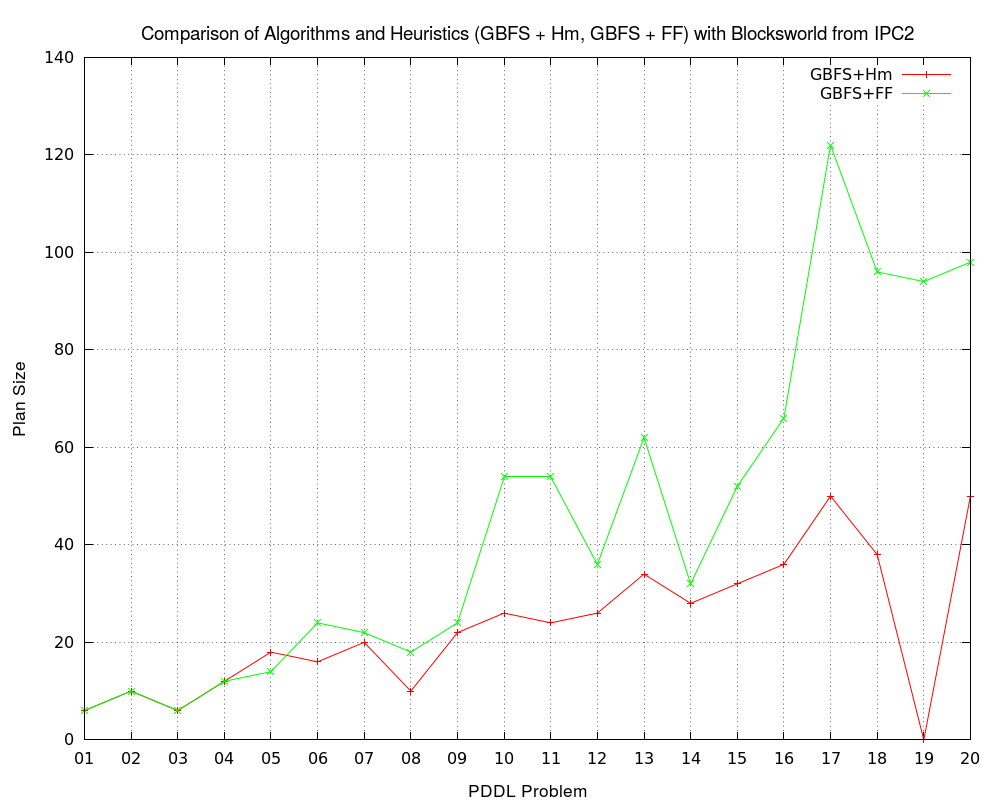
\includegraphics[scale=0.35]{BlocksworldPlanSizeGwithCP.png}
    \caption{Blocksworld domain from IPC2, GBFS with EHC + FF vs GBFS + $H^m$ }
    \label{fig:BlocksworldDomainGBFSwithHm}
\end{figure}
As the $H^m$ heuristic was only able to complete 19 out of the 35 problems within the time limit, we selected only the first 20 problems to create the graph \ref{fig:BlocksworldDomainGBFSwithHm}. Except for one instance (PDDL problem 5), the $H^m$ heuristic plan size stayed below GBFS with EHC using Fast Forward. As $H^m$ is an admissible heuristic it provided a better quality plan as it did not overestimate or under-estimate the distance from the starting node to the goal node.  
This was a good result for the Blocksworld problem but applying the same approach to Elevator from IPC2 did not provide the same set of results. 
\begin{figure}[!htb]
    \centering
    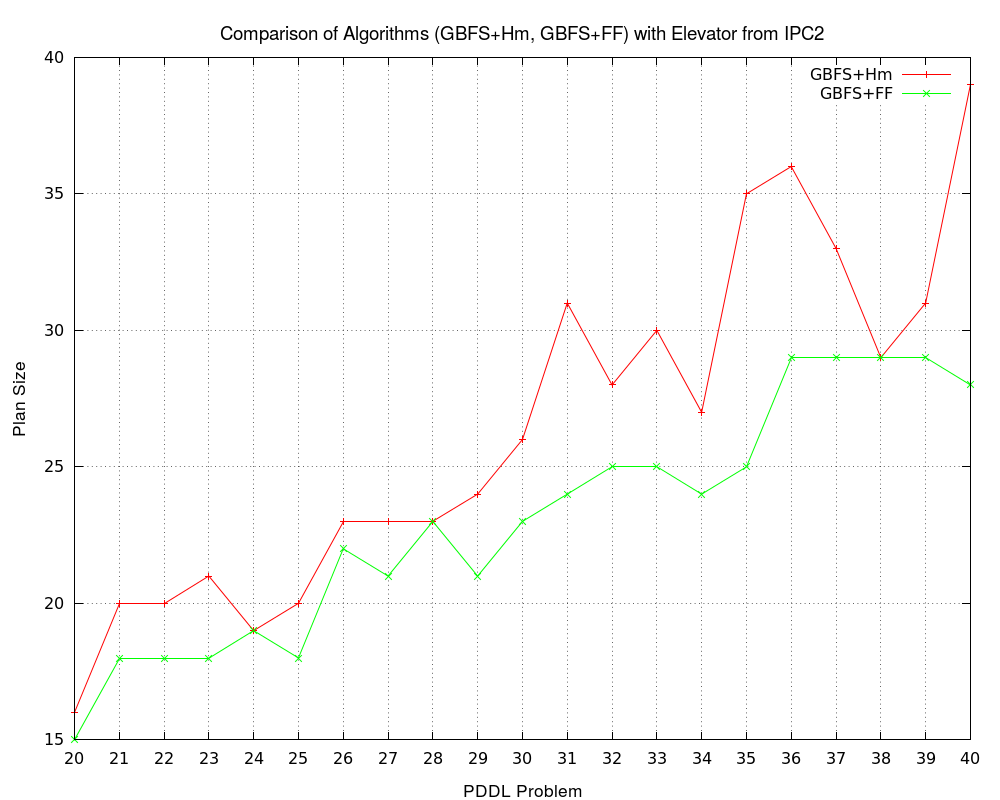
\includegraphics[scale=0.35]{Elevator20to40PlanSize.png}
    \caption{Elevator domain from IPC2, GBFS + FF vs GBFS + $H^m$ }
    \label{fig:ElevatorDomainGBFSwithHm}
\end{figure}
We can see that with some of problems, the plan size was the same but with the majority of others the plan size for $H^m$ was larger which is not what we expected given the results from the Blocksworld domain. 
\section{Test of Hypotheses}
In Chapter \ref{Chapter2}, we made hypotheses about the new search algorithm (GBFS with EHC) and the new heuristic $H^m$. With regards to the search algorithm, we devised the hypothesis that it would able to solve more problems than the current algorithm (A*). From the final results, we can say that this hypothesis is now true, as GBFS with EHC was able to solve 21 more problems than A*. It is a small number in the grand scheme of how many problems were tested but it proves that the current algorithm is not better in terms of solved problems. 
We also stated that the new algorithm would be faster and use less memory than A*. From the results presented within this chapter and the raw data, we can safely say that this is true. The results in certain domains were close but in others GBFS with EHC proved to be the more superior algorithm for classical planning.
With the new heuristic we saw that it was unable to complete more problems than the other heuristics within the library and also the speed and memory consumption was not better overall. We were able to spot some anomalies within the actions used to achieve a goal from the Blocksworld domain which suggest that the other heuristics are not using the most optimal approach when solving a problem. This concerns Max more as it is an admissible heuristic, even though it does not overestimate or under-estimate the distance to the goal, it uses actions that are possibly more costly in achieving a goal.  
\chapter{Conclusion} % Main chapter title

\label{Chapter5}

\section{Conclusion of Work}
In Chapter \ref{Chapter1} we detailed the outline that would be the general theme for the thesis, Classical Planning approaches. We provided the main aspects of classical planning and what were the topics we would be covering in the next sections. Explaining the aspects of the PDDL4J library, PDDL, Satisfiability problems and the goal for this thesis. 

We would then go on in Chapter \ref{Chapter2} to discuss what areas we will be focusing on and how we would try to achieve the goals of this thesis. We also discussed many approaches in terms of state-space planning as we felt using one of these algorithms would prove our initial hypotheses set out at the end of Chapter \ref{Chapter2}. The overall goal of Chapter \ref{Chapter2} was to grasp an understand into the world of planning, and through research, be able to come to a conclusion with what algorithms would prove our hypotheses. 

Chapter \ref{Chapter3} described how we would test the various assumptions, and based on \cite{Evaluation} how we would test the new algorithms. We also described the implementation phase of the new search algorithm and heuristic function. These were based on \cite{FFPlanner} and \cite{PlanningBook} plus \cite{HmHeuristic}. 

The last Chapter, \ref{Chapter4}, we compiled all the results from the multiple tests and discussed the results, as well as tested our hypotheses set out in Chapter \ref{Chapter2}.

In this thesis we were able to prove that A* was not the more optimal search algorithm for the PDDL4J planner, as the new search algorithm, Greedy Best First Search with Enforced Hill Climbing based on \cite{FFPlanner} was better overall. Even though there were some domains were A* was better, the more solved problems in a faster, less memory consumed manor went to GBFS with EHC. We can see by the results the difference between these two algorithms and in the next section below we discuss future additions to the algorithm and the PDDL4J planner. 

The $H^m$ heuristic on the other hand did not goes as well as expected, from the beginning we knew that it would be computationally expensive to compute but did not assume that it would not be able to solve a majority of the problems. Even though we were able to see some anomalies between actions, in the majority of harder problems in Blocksworld for example, it was unable to solve past problem 12. When paired together with the GBFS with EHC algorithm it provided the same base of results in terms of solved problems but in some of the domains the speed was worse for GBFS with EHC.  

In the following sections, we converted PDDL problems into SAT problems and gave the problems to the SAT4J library. This provided fast results in solving some of the Blocksworld problems compared to PDDL4J (A* and GBFS with EHC). Further testing would have been a plus in this area so more problems could be analysed but this has went into the future work section below as an extension to the PDDL4J planner. 
\section{Limitations}
One of the biggest limitations for me was the fact that I did not create the PDDL4J planner, which meant that I had to spend a lot of time trying to figure out such things as how it all worked, how classes linked together, what methods were available to me, etc.  This took up a large part of my time when it came to creating the two algorithms.  Also, even though Java is a very popular coding language and I have worked with it throughout my University career, some of the classes use “Bitset”, which is something I had never used before, so trying to familiarise myself with that as well as conducting research on a topic about which I know only a little was certainly challenging.
\section{Future Work} 
For future work, I feel there is a great deal that could be incorporated in the PDDL4J library that has not as yet been implemented, one of those things being the incorporation of a SAT solver, which would enable the library to solve satisfiability problems as PDDL.

Another addition could be a potential learning algorithm, one that start to build knowledge of the4 actions with a domain, meaning that the initial problems would be run as normal but the more the planner runs problems within a certain domain like Blocksworld, the more it would understand how to use actions in an optimal manner.

An algorithm that could take into account two heuristics would be good for classical planning approaches as combining a not admissible heuristic and an admissible heuristic could complement each other in certain areas. So for example, if the not admissible heuristic was stuck in a section, the admissible heuristic could take over to push past or go back from a dead end and letting the not admissible heuristic take over again. Potentially, this could provide a fast classical planner that could provide semi-optimal plans.  

%----------------------------------------------------------------------------------------
%	THESIS CONTENT - APPENDICES
%----------------------------------------------------------------------------------------
\printbibliography[heading=bibintoc]
\appendix % Cue to tell LaTeX that the following "chapters" are Appendices

% Include the appendices of the thesis as separate files from the Appendices folder
% Uncomment the lines as you write the Appendices

% Appendix A

\chapter{Appendix Title Here} % Main appendix title

\label{AppendixA}
 % For referencing this appendix elsewhere, use \ref{AppendixA}
http://github.com/aaronboyd92/MasterThesis

This is where all the raw data files, code for the search algorithm and heuristic algorithms are.

Please read the file titled 'ReadMe' which will explain the contents of the GitHub repository.

Due to the large amount of test documents, GitHub was used to provide all the results in a easy to access fashion. 
%% Appendix A

\chapter{Appendix Title Here} % Main appendix title

\label{AppendixB} % For referencing this appendix elsewhere, use \ref{AppendixA}

\section{PSR}
Checking plan: pddl01.txt
Plan to validate:
Plan size: 9
1:
(wait_cb1) 
2:
(wait_cb1-condeff0-yes) 
3:
(wait_cb1-endof-condeffs) 
4:
(open-sd2) 
5:
(open-sd1) 
6:
(close_cb1) 
7:
(wait_cb1) 
8:
(wait_cb1-condeff0-no-0) 
9:
(wait_cb1-endof-condeffs) 

Plan Validation details
-----------------------
Checking next happening (time 1)
Deleting (do-normal)
Deleting (not-updated-cb1)
Adding (do-wait_cb1-condeffs)
Adding (updated-cb1)

Checking next happening (time 2)
Deleting (closed-cb1)
Adding (done-0)
Adding (not-closed-cb1)

Checking next happening (time 3)
Deleting (do-wait_cb1-condeffs)
Deleting (done-0)
Adding (do-normal)

Checking next happening (time 4)
Deleting (closed-sd2)
Adding (not-closed-sd2)

Checking next happening (time 5)
Deleting (closed-sd1)
Adding (not-closed-sd1)

Checking next happening (time 6)
Deleting (not-closed-cb1)
Deleting (updated-cb1)
Adding (closed-cb1)
Adding (not-updated-cb1)

Checking next happening (time 7)
Deleting (do-normal)
Deleting (not-updated-cb1)
Adding (do-wait_cb1-condeffs)
Adding (updated-cb1)

Checking next happening (time 8)
Adding (done-0)

Checking next happening (time 9)
Deleting (do-wait_cb1-condeffs)
Deleting (done-0)
Adding (do-normal)
Plan executed successfully - checking goal
Plan valid
Final value: 9 

Successful plans:
Value: 9
 pddl01.txt 9 
\section{Sokoban}
Type-checking move
...action passes type checking.
Type-checking push-to-nongoal
...action passes type checking.
Type-checking push-to-goal
...action passes type checking.
Checking plan: pddl01.txt
Plan to validate:

Plan size: 41
1:
(move player-01 pos-6-4 pos-6-3 dir-up)
2:
(move player-01 pos-6-3 pos-5-3 dir-left)
3:
(move player-01 pos-5-3 pos-4-3 dir-left)
4:
(push-to-nongoal player-01 stone-02 pos-4-3 pos-4-4 pos-4-5 dir-down)
5:
(move player-01 pos-4-4 pos-4-3 dir-up)
6:
(move player-01 pos-4-3 pos-5-3 dir-right)
7:
(move player-01 pos-5-3 pos-6-3 dir-right)
8:
(move player-01 pos-6-3 pos-6-4 dir-down)
9:
(push-to-goal player-01 stone-03 pos-6-4 pos-5-4 pos-4-4 dir-left)
10:
(move player-01 pos-5-4 pos-5-3 dir-up)
11:
(move player-01 pos-5-3 pos-4-3 dir-left)
12:
(move player-01 pos-4-3 pos-3-3 dir-left)
13:
(move player-01 pos-3-3 pos-2-3 dir-left)
14:
(move player-01 pos-2-3 pos-2-4 dir-down)
15:
(move player-01 pos-2-4 pos-2-5 dir-down)
16:
(move player-01 pos-2-5 pos-3-5 dir-right)
17:
(push-to-nongoal player-01 stone-01 pos-3-5 pos-3-4 pos-3-3 dir-up)
18:
(push-to-nongoal player-01 stone-03 pos-3-4 pos-4-4 pos-5-4 dir-right)
19:
(move player-01 pos-4-4 pos-4-3 dir-up)
20:
(move player-01 pos-4-3 pos-5-3 dir-right)
21:
(move player-01 pos-5-3 pos-6-3 dir-right)
22:
(move player-01 pos-6-3 pos-6-4 dir-down)
23:
(push-to-goal player-01 stone-03 pos-6-4 pos-5-4 pos-4-4 dir-left)
24:
(push-to-goal player-01 stone-03 pos-5-4 pos-4-4 pos-3-4 dir-left)
25:
(push-to-goal player-01 stone-03 pos-4-4 pos-3-4 pos-2-4 dir-left)
26:
(move player-01 pos-3-4 pos-3-5 dir-down)
27:
(move player-01 pos-3-5 pos-3-6 dir-down)
28:
(move player-01 pos-3-6 pos-4-6 dir-right)
29:
(push-to-goal player-01 stone-02 pos-4-6 pos-4-5 pos-4-4 dir-up)
30:
(move player-01 pos-4-5 pos-3-5 dir-left)
31:
(move player-01 pos-3-5 pos-3-4 dir-up)
32:
(push-to-nongoal player-01 stone-02 pos-3-4 pos-4-4 pos-5-4 dir-right)
33:
(move player-01 pos-4-4 pos-4-3 dir-up)
34:
(move player-01 pos-4-3 pos-4-2 dir-up)
35:
(move player-01 pos-4-2 pos-3-2 dir-left)
36:
(push-to-goal player-01 stone-01 pos-3-2 pos-3-3 pos-3-4 dir-down)
37:
(move player-01 pos-3-3 pos-4-3 dir-right)
38:
(move player-01 pos-4-3 pos-5-3 dir-right)
39:
(move player-01 pos-5-3 pos-6-3 dir-right)
40:
(move player-01 pos-6-3 pos-6-4 dir-down)
41:
(push-to-goal player-01 stone-02 pos-6-4 pos-5-4 pos-4-4 dir-left)
 
Plan Validation details
-----------------------

Checking next happening (time 1)
Deleting (at player-01 pos-6-4)
Deleting (clear pos-6-3)
Adding (at player-01 pos-6-3)
Adding (clear pos-6-4)

Checking next happening (time 2)
Deleting (at player-01 pos-6-3)
Deleting (clear pos-5-3)
Adding (at player-01 pos-5-3)
Adding (clear pos-6-3)

Checking next happening (time 3)
Deleting (at player-01 pos-5-3)
Deleting (clear pos-4-3)
Adding (at player-01 pos-4-3)
Adding (clear pos-5-3)

Checking next happening (time 4)
Deleting (at player-01 pos-4-3)
Deleting (at stone-02 pos-4-4)
Deleting (clear pos-4-5)
Deleting (at-goal stone-02)
Adding (at player-01 pos-4-4)
Adding (at stone-02 pos-4-5)
Adding (clear pos-4-3)

Checking next happening (time 5)
Deleting (at player-01 pos-4-4)
Deleting (clear pos-4-3)
Adding (at player-01 pos-4-3)
Adding (clear pos-4-4)

Checking next happening (time 6)
Deleting (at player-01 pos-4-3)
Deleting (clear pos-5-3)
Adding (at player-01 pos-5-3)
Adding (clear pos-4-3)

Checking next happening (time 7)
Deleting (at player-01 pos-5-3)
Deleting (clear pos-6-3)
Adding (at player-01 pos-6-3)
Adding (clear pos-5-3)

Checking next happening (time 8)
Deleting (at player-01 pos-6-3)
Deleting (clear pos-6-4)
Adding (at player-01 pos-6-4)
Adding (clear pos-6-3)

Checking next happening (time 9)
Deleting (at player-01 pos-6-4)
Deleting (at stone-03 pos-5-4)
Deleting (clear pos-4-4)
Adding (at player-01 pos-5-4)
Adding (at stone-03 pos-4-4)
Adding (clear pos-6-4)
Adding (at-goal stone-03)

Checking next happening (time 10)
Deleting (at player-01 pos-5-4)
Deleting (clear pos-5-3)
Adding (at player-01 pos-5-3)
Adding (clear pos-5-4)

Checking next happening (time 11)
Deleting (at player-01 pos-5-3)
Deleting (clear pos-4-3)
Adding (at player-01 pos-4-3)
Adding (clear pos-5-3)

Checking next happening (time 12)
Deleting (at player-01 pos-4-3)
Deleting (clear pos-3-3)
Adding (at player-01 pos-3-3)
Adding (clear pos-4-3)

Checking next happening (time 13)
Deleting (at player-01 pos-3-3)
Deleting (clear pos-2-3)
Adding (at player-01 pos-2-3)
Adding (clear pos-3-3)

Checking next happening (time 14)
Deleting (at player-01 pos-2-3)
Deleting (clear pos-2-4)
Adding (at player-01 pos-2-4)
Adding (clear pos-2-3)

Checking next happening (time 15)
Deleting (at player-01 pos-2-4)
Deleting (clear pos-2-5)
Adding (at player-01 pos-2-5)
Adding (clear pos-2-4)

Checking next happening (time 16)
Deleting (at player-01 pos-2-5)
Deleting (clear pos-3-5)
Adding (at player-01 pos-3-5)
Adding (clear pos-2-5)

Checking next happening (time 17)
Deleting (at player-01 pos-3-5)
Deleting (at stone-01 pos-3-4)
Deleting (clear pos-3-3)
Deleting (at-goal stone-01)
Adding (at player-01 pos-3-4)
Adding (at stone-01 pos-3-3)
Adding (clear pos-3-5)

Checking next happening (time 18)
Deleting (at player-01 pos-3-4)
Deleting (at stone-03 pos-4-4)
Deleting (clear pos-5-4)
Deleting (at-goal stone-03)
Adding (at player-01 pos-4-4)
Adding (at stone-03 pos-5-4)
Adding (clear pos-3-4)

Checking next happening (time 19)
Deleting (at player-01 pos-4-4)
Deleting (clear pos-4-3)
Adding (at player-01 pos-4-3)
Adding (clear pos-4-4)

Checking next happening (time 20)
Deleting (at player-01 pos-4-3)
Deleting (clear pos-5-3)
Adding (at player-01 pos-5-3)
Adding (clear pos-4-3)

Checking next happening (time 21)
Deleting (at player-01 pos-5-3)
Deleting (clear pos-6-3)
Adding (at player-01 pos-6-3)
Adding (clear pos-5-3)

Checking next happening (time 22)
Deleting (at player-01 pos-6-3)
Deleting (clear pos-6-4)
Adding (at player-01 pos-6-4)
Adding (clear pos-6-3)

Checking next happening (time 23)
Deleting (at player-01 pos-6-4)
Deleting (at stone-03 pos-5-4)
Deleting (clear pos-4-4)
Adding (at player-01 pos-5-4)
Adding (at stone-03 pos-4-4)
Adding (clear pos-6-4)
Adding (at-goal stone-03)

Checking next happening (time 24)
Deleting (at player-01 pos-5-4)
Deleting (at stone-03 pos-4-4)
Deleting (clear pos-3-4)
Adding (at player-01 pos-4-4)
Adding (at stone-03 pos-3-4)
Adding (clear pos-5-4)
Adding (at-goal stone-03)

Checking next happening (time 25)
Deleting (at player-01 pos-4-4)
Deleting (at stone-03 pos-3-4)
Deleting (clear pos-2-4)
Adding (at player-01 pos-3-4)
Adding (at stone-03 pos-2-4)
Adding (clear pos-4-4)
Adding (at-goal stone-03)

Checking next happening (time 26)
Deleting (at player-01 pos-3-4)
Deleting (clear pos-3-5)
Adding (at player-01 pos-3-5)
Adding (clear pos-3-4)

Checking next happening (time 27)
Deleting (at player-01 pos-3-5)
Deleting (clear pos-3-6)
Adding (at player-01 pos-3-6)
Adding (clear pos-3-5)

Checking next happening (time 28)
Deleting (at player-01 pos-3-6)
Deleting (clear pos-4-6)
Adding (at player-01 pos-4-6)
Adding (clear pos-3-6)

Checking next happening (time 29)
Deleting (at player-01 pos-4-6)
Deleting (at stone-02 pos-4-5)
Deleting (clear pos-4-4)
Adding (at player-01 pos-4-5)
Adding (at stone-02 pos-4-4)
Adding (clear pos-4-6)
Adding (at-goal stone-02)

Checking next happening (time 30)
Deleting (at player-01 pos-4-5)
Deleting (clear pos-3-5)
Adding (at player-01 pos-3-5)
Adding (clear pos-4-5)

Checking next happening (time 31)
Deleting (at player-01 pos-3-5)
Deleting (clear pos-3-4)
Adding (at player-01 pos-3-4)
Adding (clear pos-3-5)

Checking next happening (time 32)
Deleting (at player-01 pos-3-4)
Deleting (at stone-02 pos-4-4)
Deleting (clear pos-5-4)
Deleting (at-goal stone-02)
Adding (at player-01 pos-4-4)
Adding (at stone-02 pos-5-4)
Adding (clear pos-3-4)

Checking next happening (time 33)
Deleting (at player-01 pos-4-4)
Deleting (clear pos-4-3)
Adding (at player-01 pos-4-3)
Adding (clear pos-4-4)

Checking next happening (time 34)
Deleting (at player-01 pos-4-3)
Deleting (clear pos-4-2)
Adding (at player-01 pos-4-2)
Adding (clear pos-4-3)

Checking next happening (time 35)
Deleting (at player-01 pos-4-2)
Deleting (clear pos-3-2)
Adding (at player-01 pos-3-2)
Adding (clear pos-4-2)

Checking next happening (time 36)
Deleting (at player-01 pos-3-2)
Deleting (at stone-01 pos-3-3)
Deleting (clear pos-3-4)
Adding (at player-01 pos-3-3)
Adding (at stone-01 pos-3-4)
Adding (clear pos-3-2)
Adding (at-goal stone-01)

Checking next happening (time 37)
Deleting (at player-01 pos-3-3)
Deleting (clear pos-4-3)
Adding (at player-01 pos-4-3)
Adding (clear pos-3-3)

Checking next happening (time 38)
Deleting (at player-01 pos-4-3)
Deleting (clear pos-5-3)
Adding (at player-01 pos-5-3)
Adding (clear pos-4-3)

Checking next happening (time 39)
Deleting (at player-01 pos-5-3)
Deleting (clear pos-6-3)
Adding (at player-01 pos-6-3)
Adding (clear pos-5-3)

Checking next happening (time 40)
Deleting (at player-01 pos-6-3)
Deleting (clear pos-6-4)
Adding (at player-01 pos-6-4)
Adding (clear pos-6-3)

Checking next happening (time 41)
Deleting (at player-01 pos-6-4)
Deleting (at stone-02 pos-5-4)
Deleting (clear pos-4-4)
Adding (at player-01 pos-5-4)
Adding (at stone-02 pos-4-4)
Adding (clear pos-6-4)
Adding (at-goal stone-02)
Plan executed successfully - checking goal
Plan valid
Final value: 41 

Successful plans:
Value: 41
 pddl01.txt 41 
\section{Blocksworld}
Type-checking pick-up
...action passes type checking.
Type-checking put-down
...action passes type checking.
Type-checking stack
...action passes type checking.
Type-checking unstack
...action passes type checking.
Checking plan: pddl20.txt
Plan to validate:

Plan size: 98
1:
(unstack f d)
2:
(put-down f)
3:
(unstack d h)
4:
(stack d f)
5:
(unstack c g)
6:
(stack c h)
7:
(unstack g e)
8:
(put-down g)
9:
(unstack e i)
10:
(put-down e)
11:
(unstack i j)
12:
(stack i d)
13:
(pick-up g)
14:
(stack g j)
15:
(unstack i d)
16:
(put-down i)
17:
(unstack c h) 
18:
(stack c d) 
19:
(pick-up i) 
20:
(stack i c) 
21:
(pick-up e) 
22:
(stack e h) 
23:
(unstack i c) 
24:
(put-down i) 
25:
(unstack c d) 
26:
(put-down c) 
27:
(pick-up i) 
28:
(stack i d) 
29:
(pick-up c) 
30:
(stack c g) 
31:
(unstack i d) 
32:
(stack i c) 
33:
(unstack d f) 
34:
(put-down d) 
35:
(unstack i c) 
36:
(put-down i) 
37:
(pick-up f) 
38:
(stack f i) 
39:
(pick-up d) 
40:
(stack d f) 
41:
(unstack c g) 
42:
(put-down c) 
43:
(unstack g j) 
44:
(put-down g) 
45:
(unstack j a) 
46:
(put-down j) 
47:
(unstack a b) 
48:
(stack a e) 
49:
(pick-up b) 
50:
(stack b d) 
51:
(pick-up c) 
52:
(stack c b) 
53:
(pick-up g) 
54:
(stack g j) 
55:
(unstack a e) 
56:
(stack a c) 
57:
(unstack e h) 
58:
(put-down e) 
59:
(pick-up h) 
60:
(stack h g) 
61:
(pick-up e) 
62:
(stack e h) 
63:
(unstack a c) 
64:
(stack a e) 
65:
(unstack c b) 
66:
(put-down c) 
67:
(unstack b d) 
68:
(put-down b) 
69:
(pick-up c) 
70:
(stack c b) 
71:
(unstack d f) 
72:
(put-down d) 
73:
(unstack c b) 
74:
(put-down c) 
75:
(pick-up b) 
76:
(stack b d) 
77:
(pick-up c) 
78:
(stack c b) 
79:
(unstack f i) 
80:
(put-down f) 
81:
(pick-up i) 
82:
(stack i a) 
83:
(pick-up f) 
84:
(stack f i) 
85:
(unstack c b) 
86:
(put-down c) 
87:
(unstack b d) 
88:
(put-down b) 
89:
(pick-up c) 
90:
(stack c b) 
91:
(pick-up d) 
92:
(stack d f) 
93:
(unstack c b) 
94:
(put-down c) 
95:
(pick-up b) 
96:
(stack b d) 
97:
(pick-up c) 
98:
(stack c b) 

Plan Validation details
-----------------------

Checking next happening (time 1)
Deleting (clear f)
Deleting (handempty)
Deleting (on f d)
Adding (holding f)
Adding (clear d)

Checking next happening (time 2)
Deleting (holding f)
Adding (clear f)
Adding (handempty)
Adding (ontable f)

Checking next happening (time 3)
Deleting (clear d)
Deleting (handempty)
Deleting (on d h)
Adding (holding d)
Adding (clear h)

Checking next happening (time 4)
Deleting (holding d)
Deleting (clear f)
Adding (clear d)
Adding (handempty)
Adding (on d f)

Checking next happening (time 5)
Deleting (clear c)
Deleting (handempty)
Deleting (on c g)
Adding (holding c)
Adding (clear g)

Checking next happening (time 6)
Deleting (holding c)
Deleting (clear h)
Adding (clear c)
Adding (handempty)
Adding (on c h)

Checking next happening (time 7)
Deleting (clear g)
Deleting (handempty)
Deleting (on g e)
Adding (holding g)
Adding (clear e)

Checking next happening (time 8)
Deleting (holding g)
Adding (clear g)
Adding (handempty)
Adding (ontable g)

Checking next happening (time 9)
Deleting (clear e)
Deleting (handempty)
Deleting (on e i)
Adding (holding e)
Adding (clear i)

Checking next happening (time 10)
Deleting (holding e)
Adding (clear e)
Adding (handempty)
Adding (ontable e)

Checking next happening (time 11)
Deleting (clear i)
Deleting (handempty)
Deleting (on i j)
Adding (holding i)
Adding (clear j)

Checking next happening (time 12)
Deleting (holding i)
Deleting (clear d)
Adding (clear i)
Adding (handempty)
Adding (on i d)

Checking next happening (time 13)
Deleting (ontable g)
Deleting (clear g)
Deleting (handempty)
Adding (holding g)

Checking next happening (time 14)
Deleting (holding g)
Deleting (clear j)
Adding (clear g)
Adding (handempty)
Adding (on g j)

Checking next happening (time 15)
Deleting (clear i)
Deleting (handempty)
Deleting (on i d)
Adding (holding i)
Adding (clear d)

Checking next happening (time 16)
Deleting (holding i)
Adding (clear i)
Adding (handempty)
Adding (ontable i)

Checking next happening (time 17)
Deleting (clear c)
Deleting (handempty)
Deleting (on c h)
Adding (holding c)
Adding (clear h)

Checking next happening (time 18)
Deleting (holding c)
Deleting (clear d)
Adding (clear c)
Adding (handempty)
Adding (on c d)

Checking next happening (time 19)
Deleting (ontable i)
Deleting (clear i)
Deleting (handempty)
Adding (holding i)

Checking next happening (time 20)
Deleting (holding i)
Deleting (clear c)
Adding (clear i)
Adding (handempty)
Adding (on i c)

Checking next happening (time 21)
Deleting (ontable e)
Deleting (clear e)
Deleting (handempty)
Adding (holding e)

Checking next happening (time 22)
Deleting (holding e)
Deleting (clear h)
Adding (clear e)
Adding (handempty)
Adding (on e h)

Checking next happening (time 23)
Deleting (clear i)
Deleting (handempty)
Deleting (on i c)
Adding (holding i)
Adding (clear c)

Checking next happening (time 24)
Deleting (holding i)
Adding (clear i)
Adding (handempty)
Adding (ontable i)

Checking next happening (time 25)
Deleting (clear c)
Deleting (handempty)
Deleting (on c d)
Adding (holding c)
Adding (clear d)

Checking next happening (time 26)
Deleting (holding c)
Adding (clear c)
Adding (handempty)
Adding (ontable c)

Checking next happening (time 27)
Deleting (ontable i)
Deleting (clear i)
Deleting (handempty)
Adding (holding i)

Checking next happening (time 28)
Deleting (holding i)
Deleting (clear d)
Adding (clear i)
Adding (handempty)
Adding (on i d)

Checking next happening (time 29)
Deleting (ontable c)
Deleting (clear c)
Deleting (handempty)
Adding (holding c)

Checking next happening (time 30)
Deleting (holding c)
Deleting (clear g)
Adding (clear c)
Adding (handempty)
Adding (on c g)

Checking next happening (time 31)
Deleting (clear i)
Deleting (handempty)
Deleting (on i d)
Adding (holding i)
Adding (clear d)

Checking next happening (time 32)
Deleting (holding i)
Deleting (clear c)
Adding (clear i)
Adding (handempty)
Adding (on i c)

Checking next happening (time 33)
Deleting (clear d)
Deleting (handempty)
Deleting (on d f)
Adding (holding d)
Adding (clear f)

Checking next happening (time 34)
Deleting (holding d)
Adding (clear d)
Adding (handempty)
Adding (ontable d)

Checking next happening (time 35)
Deleting (clear i)
Deleting (handempty)
Deleting (on i c)
Adding (holding i)
Adding (clear c)

Checking next happening (time 36)
Deleting (holding i)
Adding (clear i)
Adding (handempty)
Adding (ontable i)

Checking next happening (time 37)
Deleting (ontable f)
Deleting (clear f)
Deleting (handempty)
Adding (holding f)

Checking next happening (time 38)
Deleting (holding f)
Deleting (clear i)
Adding (clear f)
Adding (handempty)
Adding (on f i)

Checking next happening (time 39)
Deleting (ontable d)
Deleting (clear d)
Deleting (handempty)
Adding (holding d)

Checking next happening (time 40)
Deleting (holding d)
Deleting (clear f)
Adding (clear d)
Adding (handempty)
Adding (on d f)

Checking next happening (time 41)
Deleting (clear c)
Deleting (handempty)
Deleting (on c g)
Adding (holding c)
Adding (clear g)

Checking next happening (time 42)
Deleting (holding c)
Adding (clear c)
Adding (handempty)
Adding (ontable c)

Checking next happening (time 43)
Deleting (clear g)
Deleting (handempty)
Deleting (on g j)
Adding (holding g)
Adding (clear j)

Checking next happening (time 44)
Deleting (holding g)
Adding (clear g)
Adding (handempty)
Adding (ontable g)

Checking next happening (time 45)
Deleting (clear j)
Deleting (handempty)
Deleting (on j a)
Adding (holding j)
Adding (clear a)

Checking next happening (time 46)
Deleting (holding j)
Adding (clear j)
Adding (handempty)
Adding (ontable j)

Checking next happening (time 47)
Deleting (clear a)
Deleting (handempty)
Deleting (on a b)
Adding (holding a)
Adding (clear b)

Checking next happening (time 48)
Deleting (holding a)
Deleting (clear e)
Adding (clear a)
Adding (handempty)
Adding (on a e)

Checking next happening (time 49)
Deleting (ontable b)
Deleting (clear b)
Deleting (handempty)
Adding (holding b)

Checking next happening (time 50)
Deleting (holding b)
Deleting (clear d)
Adding (clear b)
Adding (handempty)
Adding (on b d)

Checking next happening (time 51)
Deleting (ontable c)
Deleting (clear c)
Deleting (handempty)
Adding (holding c)

Checking next happening (time 52)
Deleting (holding c)
Deleting (clear b)
Adding (clear c)
Adding (handempty)
Adding (on c b)

Checking next happening (time 53)
Deleting (ontable g)
Deleting (clear g)
Deleting (handempty)
Adding (holding g)

Checking next happening (time 54)
Deleting (holding g)
Deleting (clear j)
Adding (clear g)
Adding (handempty)
Adding (on g j)

Checking next happening (time 55)
Deleting (clear a)
Deleting (handempty)
Deleting (on a e)
Adding (holding a)
Adding (clear e)

Checking next happening (time 56)
Deleting (holding a)
Deleting (clear c)
Adding (clear a)
Adding (handempty)
Adding (on a c)

Checking next happening (time 57)
Deleting (clear e)
Deleting (handempty)
Deleting (on e h)
Adding (holding e)
Adding (clear h)

Checking next happening (time 58)
Deleting (holding e)
Adding (clear e)
Adding (handempty)
Adding (ontable e)

Checking next happening (time 59)
Deleting (ontable h)
Deleting (clear h)
Deleting (handempty)
Adding (holding h)

Checking next happening (time 60)
Deleting (holding h)
Deleting (clear g)
Adding (clear h)
Adding (handempty)
Adding (on h g)

Checking next happening (time 61)
Deleting (ontable e)
Deleting (clear e)
Deleting (handempty)
Adding (holding e)

Checking next happening (time 62)
Deleting (holding e)
Deleting (clear h)
Adding (clear e)
Adding (handempty)
Adding (on e h)

Checking next happening (time 63)
Deleting (clear a)
Deleting (handempty)
Deleting (on a c)
Adding (holding a)
Adding (clear c)

Checking next happening (time 64)
Deleting (holding a)
Deleting (clear e)
Adding (clear a)
Adding (handempty)
Adding (on a e)

Checking next happening (time 65)
Deleting (clear c)
Deleting (handempty)
Deleting (on c b)
Adding (holding c)
Adding (clear b)

Checking next happening (time 66)
Deleting (holding c)
Adding (clear c)
Adding (handempty)
Adding (ontable c)

Checking next happening (time 67)
Deleting (clear b)
Deleting (handempty)
Deleting (on b d)
Adding (holding b)
Adding (clear d)

Checking next happening (time 68)
Deleting (holding b)
Adding (clear b)
Adding (handempty)
Adding (ontable b)

Checking next happening (time 69)
Deleting (ontable c)
Deleting (clear c)
Deleting (handempty)
Adding (holding c)

Checking next happening (time 70)
Deleting (holding c)
Deleting (clear b)
Adding (clear c)
Adding (handempty)
Adding (on c b)

Checking next happening (time 71)
Deleting (clear d)
Deleting (handempty)
Deleting (on d f)
Adding (holding d)
Adding (clear f)

Checking next happening (time 72)
Deleting (holding d)
Adding (clear d)
Adding (handempty)
Adding (ontable d)

Checking next happening (time 73)
Deleting (clear c)
Deleting (handempty)
Deleting (on c b)
Adding (holding c)
Adding (clear b)

Checking next happening (time 74)
Deleting (holding c)
Adding (clear c)
Adding (handempty)
Adding (ontable c)

Checking next happening (time 75)
Deleting (ontable b)
Deleting (clear b)
Deleting (handempty)
Adding (holding b)

Checking next happening (time 76)
Deleting (holding b)
Deleting (clear d)
Adding (clear b)
Adding (handempty)
Adding (on b d)

Checking next happening (time 77)
Deleting (ontable c)
Deleting (clear c)
Deleting (handempty)
Adding (holding c)

Checking next happening (time 78)
Deleting (holding c)
Deleting (clear b)
Adding (clear c)
Adding (handempty)
Adding (on c b)

Checking next happening (time 79)
Deleting (clear f)
Deleting (handempty)
Deleting (on f i)
Adding (holding f)
Adding (clear i)

Checking next happening (time 80)
Deleting (holding f)
Adding (clear f)
Adding (handempty)
Adding (ontable f)

Checking next happening (time 81)
Deleting (ontable i)
Deleting (clear i)
Deleting (handempty)
Adding (holding i)

Checking next happening (time 82)
Deleting (holding i)
Deleting (clear a)
Adding (clear i)
Adding (handempty)
Adding (on i a)

Checking next happening (time 83)
Deleting (ontable f)
Deleting (clear f)
Deleting (handempty)
Adding (holding f)

Checking next happening (time 84)
Deleting (holding f)
Deleting (clear i)
Adding (clear f)
Adding (handempty)
Adding (on f i)

Checking next happening (time 85)
Deleting (clear c)
Deleting (handempty)
Deleting (on c b)
Adding (holding c)
Adding (clear b)

Checking next happening (time 86)
Deleting (holding c)
Adding (clear c)
Adding (handempty)
Adding (ontable c)

Checking next happening (time 87)
Deleting (clear b)
Deleting (handempty)
Deleting (on b d)
Adding (holding b)
Adding (clear d)

Checking next happening (time 88)
Deleting (holding b)
Adding (clear b)
Adding (handempty)
Adding (ontable b)

Checking next happening (time 89)
Deleting (ontable c)
Deleting (clear c)
Deleting (handempty)
Adding (holding c)

Checking next happening (time 90)
Deleting (holding c)
Deleting (clear b)
Adding (clear c)
Adding (handempty)
Adding (on c b)

Checking next happening (time 91)
Deleting (ontable d)
Deleting (clear d)
Deleting (handempty)
Adding (holding d)

Checking next happening (time 92)
Deleting (holding d)
Deleting (clear f)
Adding (clear d)
Adding (handempty)
Adding (on d f)

Checking next happening (time 93)
Deleting (clear c)
Deleting (handempty)
Deleting (on c b)
Adding (holding c)
Adding (clear b)

Checking next happening (time 94)
Deleting (holding c)
Adding (clear c)
Adding (handempty)
Adding (ontable c)

Checking next happening (time 95)
Deleting (ontable b)
Deleting (clear b)
Deleting (handempty)
Adding (holding b)

Checking next happening (time 96)
Deleting (holding b)
Deleting (clear d)
Adding (clear b)
Adding (handempty)
Adding (on b d)

Checking next happening (time 97)
Deleting (ontable c)
Deleting (clear c)
Deleting (handempty)
Adding (holding c)

Checking next happening (time 98)
Deleting (holding c)
Deleting (clear b)
Adding (clear c)
Adding (handempty)
Adding (on c b)
Plan executed successfully - checking goal
Plan valid
Final value: 98 

Successful plans:
Value: 98
 pddl20.txt 98 

Type-checking pick-up
...action passes type checking.
Type-checking put-down
...action passes type checking.
Type-checking stack
...action passes type checking.
Type-checking unstack
...action passes type checking.
Checking plan: pddl10.txt
Plan to validate:

Plan size: 54
1:
(unstack e g) 
2:
(put-down e) 
3:
(unstack g b) 
4:
(put-down g) 
5:
(unstack b a) 
6:
(stack b e) 
7:
(unstack a f) 
8:
(stack a g) 
9:
(unstack f c) 
10:
(put-down f) 
11:
(unstack c d) 
12:
(stack c f) 
13:
(unstack b e) 
14:
(stack b c) 
15:
(pick-up d) 
16:
(stack d e) 
17:
(unstack b c) 
18:
(put-down b) 
19:
(unstack d e) 
20:
(stack d b) 
21:
(unstack a g) 
22:
(stack a e) 
23:
(pick-up g) 
24:
(stack g d) 
25:
(unstack a e) 
26:
(stack a g) 
27:
(unstack c f) 
28:
(stack c e) 
29:
(pick-up f) 
30:
(stack f a) 
31:
(unstack c e) 
32:
(put-down c) 
33:
(unstack f a) 
34:
(stack f e) 
35:
(pick-up c) 
36:
(stack c f) 
37:
(unstack a g) 
38:
(put-down a) 
39:
(unstack g d) 
40:
(put-down g) 
41:
(pick-up a) 
42:
(stack a g) 
43:
(unstack d b) 
44:
(put-down d) 
45:
(pick-up b) 
46:
(stack b c) 
47:
(pick-up d) 
48:
(stack d b) 
49:
(unstack a g) 
50:
(put-down a) 
51:
(pick-up g) 
52:
(stack g d) 
53:
(pick-up a) 
54:
(stack a g) 

Plan Validation details
-----------------------

Checking next happening (time 1)
Deleting (clear e)
Deleting (handempty)
Deleting (on e g)
Adding (holding e)
Adding (clear g)

Checking next happening (time 2)
Deleting (holding e)
Adding (clear e)
Adding (handempty)
Adding (ontable e)

Checking next happening (time 3)
Deleting (clear g)
Deleting (handempty)
Deleting (on g b)
Adding (holding g)
Adding (clear b)

Checking next happening (time 4)
Deleting (holding g)
Adding (clear g)
Adding (handempty)
Adding (ontable g)

Checking next happening (time 5)
Deleting (clear b)
Deleting (handempty)
Deleting (on b a)
Adding (holding b)
Adding (clear a)

Checking next happening (time 6)
Deleting (holding b)
Deleting (clear e)
Adding (clear b)
Adding (handempty)
Adding (on b e)

Checking next happening (time 7)
Deleting (clear a)
Deleting (handempty)
Deleting (on a f)
Adding (holding a)
Adding (clear f)

Checking next happening (time 8)
Deleting (holding a)
Deleting (clear g)
Adding (clear a)
Adding (handempty)
Adding (on a g)

Checking next happening (time 9)
Deleting (clear f)
Deleting (handempty)
Deleting (on f c)
Adding (holding f)
Adding (clear c)

Checking next happening (time 10)
Deleting (holding f)
Adding (clear f)
Adding (handempty)
Adding (ontable f)

Checking next happening (time 11)
Deleting (clear c)
Deleting (handempty)
Deleting (on c d)
Adding (holding c)
Adding (clear d)

Checking next happening (time 12)
Deleting (holding c)
Deleting (clear f)
Adding (clear c)
Adding (handempty)
Adding (on c f)

Checking next happening (time 13)
Deleting (clear b)
Deleting (handempty)
Deleting (on b e)
Adding (holding b)
Adding (clear e)

Checking next happening (time 14)
Deleting (holding b)
Deleting (clear c)
Adding (clear b)
Adding (handempty)
Adding (on b c)

Checking next happening (time 15)
Deleting (ontable d)
Deleting (clear d)
Deleting (handempty)
Adding (holding d)

Checking next happening (time 16)
Deleting (holding d)
Deleting (clear e)
Adding (clear d)
Adding (handempty)
Adding (on d e)

Checking next happening (time 17)
Deleting (clear b)
Deleting (handempty)
Deleting (on b c)
Adding (holding b)
Adding (clear c)

Checking next happening (time 18)
Deleting (holding b)
Adding (clear b)
Adding (handempty)
Adding (ontable b)

Checking next happening (time 19)
Deleting (clear d)
Deleting (handempty)
Deleting (on d e)
Adding (holding d)
Adding (clear e)

Checking next happening (time 20)
Deleting (holding d)
Deleting (clear b)
Adding (clear d)
Adding (handempty)
Adding (on d b)

Checking next happening (time 21)
Deleting (clear a)
Deleting (handempty)
Deleting (on a g)
Adding (holding a)
Adding (clear g)

Checking next happening (time 22)
Deleting (holding a)
Deleting (clear e)
Adding (clear a)
Adding (handempty)
Adding (on a e)

Checking next happening (time 23)
Deleting (ontable g)
Deleting (clear g)
Deleting (handempty)
Adding (holding g)

Checking next happening (time 24)
Deleting (holding g)
Deleting (clear d)
Adding (clear g)
Adding (handempty)
Adding (on g d)

Checking next happening (time 25)
Deleting (clear a)
Deleting (handempty)
Deleting (on a e)
Adding (holding a)
Adding (clear e)

Checking next happening (time 26)
Deleting (holding a)
Deleting (clear g)
Adding (clear a)
Adding (handempty)
Adding (on a g)

Checking next happening (time 27)
Deleting (clear c)
Deleting (handempty)
Deleting (on c f)
Adding (holding c)
Adding (clear f)

Checking next happening (time 28)
Deleting (holding c)
Deleting (clear e)
Adding (clear c)
Adding (handempty)
Adding (on c e)

Checking next happening (time 29)
Deleting (ontable f)
Deleting (clear f)
Deleting (handempty)
Adding (holding f)

Checking next happening (time 30)
Deleting (holding f)
Deleting (clear a)
Adding (clear f)
Adding (handempty)
Adding (on f a)

Checking next happening (time 31)
Deleting (clear c)
Deleting (handempty)
Deleting (on c e)
Adding (holding c)
Adding (clear e)

Checking next happening (time 32)
Deleting (holding c)
Adding (clear c)
Adding (handempty)
Adding (ontable c)

Checking next happening (time 33)
Deleting (clear f)
Deleting (handempty)
Deleting (on f a)
Adding (holding f)
Adding (clear a)

Checking next happening (time 34)
Deleting (holding f)
Deleting (clear e)
Adding (clear f)
Adding (handempty)
Adding (on f e)

Checking next happening (time 35)
Deleting (ontable c)
Deleting (clear c)
Deleting (handempty)
Adding (holding c)

Checking next happening (time 36)
Deleting (holding c)
Deleting (clear f)
Adding (clear c)
Adding (handempty)
Adding (on c f)

Checking next happening (time 37)
Deleting (clear a)
Deleting (handempty)
Deleting (on a g)
Adding (holding a)
Adding (clear g)

Checking next happening (time 38)
Deleting (holding a)
Adding (clear a)
Adding (handempty)
Adding (ontable a)

Checking next happening (time 39)
Deleting (clear g)
Deleting (handempty)
Deleting (on g d)
Adding (holding g)
Adding (clear d)

Checking next happening (time 40)
Deleting (holding g)
Adding (clear g)
Adding (handempty)
Adding (ontable g)

Checking next happening (time 41)
Deleting (ontable a)
Deleting (clear a)
Deleting (handempty)
Adding (holding a)

Checking next happening (time 42)
Deleting (holding a)
Deleting (clear g)
Adding (clear a)
Adding (handempty)
Adding (on a g)

Checking next happening (time 43)
Deleting (clear d)
Deleting (handempty)
Deleting (on d b)
Adding (holding d)
Adding (clear b)

Checking next happening (time 44)
Deleting (holding d)
Adding (clear d)
Adding (handempty)
Adding (ontable d)

Checking next happening (time 45)
Deleting (ontable b)
Deleting (clear b)
Deleting (handempty)
Adding (holding b)

Checking next happening (time 46)
Deleting (holding b)
Deleting (clear c)
Adding (clear b)
Adding (handempty)
Adding (on b c)

Checking next happening (time 47)
Deleting (ontable d)
Deleting (clear d)
Deleting (handempty)
Adding (holding d)

Checking next happening (time 48)
Deleting (holding d)
Deleting (clear b)
Adding (clear d)
Adding (handempty)
Adding (on d b)

Checking next happening (time 49)
Deleting (clear a)
Deleting (handempty)
Deleting (on a g)
Adding (holding a)
Adding (clear g)

Checking next happening (time 50)
Deleting (holding a)
Adding (clear a)
Adding (handempty)
Adding (ontable a)

Checking next happening (time 51)
Deleting (ontable g)
Deleting (clear g)
Deleting (handempty)
Adding (holding g)

Checking next happening (time 52)
Deleting (holding g)
Deleting (clear d)
Adding (clear g)
Adding (handempty)
Adding (on g d)

Checking next happening (time 53)
Deleting (ontable a)
Deleting (clear a)
Deleting (handempty)
Adding (holding a)

Checking next happening (time 54)
Deleting (holding a)
Deleting (clear g)
Adding (clear a)
Adding (handempty)
Adding (on a g)
Plan executed successfully - checking goal
Plan valid
Final value: 54 

Successful plans:
Value: 54
 pddl10.txt 54 
\section{Zenotravel}
Type-checking board
...action passes type checking.
Type-checking debark
...action passes type checking.
Type-checking fly
...action passes type checking.
Type-checking zoom
...action passes type checking.
Type-checking refuel
...action passes type checking.
Checking plan: pddl10.txt
Plan to validate:

Plan size: 31
1:
(zoom plane1 city0 city2 fl2 fl1 fl0)
2:
(board person4 plane2 city4)
3:
(board person3 plane2 city4)
4:
(zoom plane3 city2 city3 fl2 fl1 fl0)
5:
(zoom plane2 city4 city1 fl5 fl4 fl3)
6:
(debark person4 plane2 city1)
7:
(board person5 plane2 city1) 
8:
(board person7 plane2 city1) 
9:
(zoom plane2 city1 city0 fl3 fl2 fl1)
10:
(debark person5 plane2 city0)
11:
(board person8 plane2 city0)
12:
(board person6 plane2 city0)
13:
(refuel plane2 city0 fl1 fl2)
14:
(fly plane2 city0 city1 fl2 fl1)
15:
(refuel plane2 city1 fl1 fl2)
16:
(refuel plane2 city1 fl2 fl3)
17:
(board person2 plane3 city3)
18:
(refuel plane2 city1 fl3 fl4)
19:
(refuel plane3 city3 fl0 fl1)
20:
(fly plane3 city3 city2 fl1 fl0)
21:
(debark person2 plane3 city2)
22:
(refuel plane2 city1 fl4 fl5)
23:
(fly plane2 city1 city3 fl5 fl4)
24:
(debark person3 plane2 city3)
25:
(debark person6 plane2 city3)
26:
(debark person8 plane2 city3)
27:
(board person1 plane2 city3)
28:
(zoom plane2 city3 city1 fl4 fl3 fl2)
29:
(debark person1 plane2 city1)
30:
(fly plane2 city1 city4 fl2 fl1)
31:
(debark person7 plane2 city4)

Plan Validation details
-----------------------

Checking next happening (time 1)
Deleting (at plane1 city0)
Deleting (fuel-level plane1 fl2)
Adding (at plane1 city2)
Adding (fuel-level plane1 fl0)

Checking next happening (time 2)
Deleting (at person4 city4)
Adding (in person4 plane2)

Checking next happening (time 3)
Deleting (at person3 city4)
Adding (in person3 plane2)

Checking next happening (time 4)
Deleting (at plane3 city2)
Deleting (fuel-level plane3 fl2)
Adding (at plane3 city3)
Adding (fuel-level plane3 fl0)

Checking next happening (time 5)
Deleting (at plane2 city4)
Deleting (fuel-level plane2 fl5)
Adding (at plane2 city1)
Adding (fuel-level plane2 fl3)

Checking next happening (time 6)
Deleting (in person4 plane2)
Adding (at person4 city1)

Checking next happening (time 7)
Deleting (at person5 city1)
Adding (in person5 plane2)

Checking next happening (time 8)
Deleting (at person7 city1)
Adding (in person7 plane2)

Checking next happening (time 9)
Deleting (at plane2 city1)
Deleting (fuel-level plane2 fl3)
Adding (at plane2 city0)
Adding (fuel-level plane2 fl1)

Checking next happening (time 10)
Deleting (in person5 plane2)
Adding (at person5 city0)

Checking next happening (time 11)
Deleting (at person8 city0)
Adding (in person8 plane2)

Checking next happening (time 12)
Deleting (at person6 city0)
Adding (in person6 plane2)

Checking next happening (time 13)
Deleting (fuel-level plane2 fl1)
Adding (fuel-level plane2 fl2)

Checking next happening (time 14)
Deleting (at plane2 city0)
Deleting (fuel-level plane2 fl2)
Adding (at plane2 city1)
Adding (fuel-level plane2 fl1)

Checking next happening (time 15)
Deleting (fuel-level plane2 fl1)
Adding (fuel-level plane2 fl2)

Checking next happening (time 16)
Deleting (fuel-level plane2 fl2)
Adding (fuel-level plane2 fl3)

Checking next happening (time 17)
Deleting (at person2 city3)
Adding (in person2 plane3)

Checking next happening (time 18)
Deleting (fuel-level plane2 fl3)
Adding (fuel-level plane2 fl4)

Checking next happening (time 19)
Deleting (fuel-level plane3 fl0)
Adding (fuel-level plane3 fl1)

Checking next happening (time 20)
Deleting (at plane3 city3)
Deleting (fuel-level plane3 fl1)
Adding (at plane3 city2)
Adding (fuel-level plane3 fl0)

Checking next happening (time 21)
Deleting (in person2 plane3)
Adding (at person2 city2)

Checking next happening (time 22)
Deleting (fuel-level plane2 fl4)
Adding (fuel-level plane2 fl5)

Checking next happening (time 23)
Deleting (at plane2 city1)
Deleting (fuel-level plane2 fl5)
Adding (at plane2 city3)
Adding (fuel-level plane2 fl4)

Checking next happening (time 24)
Deleting (in person3 plane2)
Adding (at person3 city3)

Checking next happening (time 25)
Deleting (in person6 plane2)
Adding (at person6 city3)

Checking next happening (time 26)
Deleting (in person8 plane2)
Adding (at person8 city3)

Checking next happening (time 27)
Deleting (at person1 city3)
Adding (in person1 plane2)

Checking next happening (time 28)
Deleting (at plane2 city3)
Deleting (fuel-level plane2 fl4)
Adding (at plane2 city1)
Adding (fuel-level plane2 fl2)

Checking next happening (time 29)
Deleting (in person1 plane2)
Adding (at person1 city1)

Checking next happening (time 30)
Deleting (at plane2 city1)
Deleting (fuel-level plane2 fl2)
Adding (at plane2 city4)
Adding (fuel-level plane2 fl1)

Checking next happening (time 31)
Deleting (in person7 plane2)
Adding (at person7 city4)
Plan executed successfully - checking goal
Plan valid
Final value: 31 

Successful plans:
Value: 31
 pddl10.txt 31 

%\include{Appendices/AppendixC}

%----------------------------------------------------------------------------------------
%	BIBLIOGRAPHY
%----------------------------------------------------------------------------------------




\end{document}